\documentclass[11pt,letterpaper]{article}

\usepackage[utf8]{inputenc}
\usepackage[T1]{fontenc}
\usepackage[margin=1in]{geometry}
\usepackage{amsmath,amssymb}
\usepackage{graphicx}
\usepackage{hyperref}
\usepackage{xcolor}
\usepackage{booktabs}
\usepackage{enumitem}
\usepackage{caption}
\usepackage{titling}
\usepackage{fancyhdr}
\usepackage{setspace}

\hypersetup{
    colorlinks=true,
    linkcolor=black,
    citecolor=black,
    urlcolor=black,
    pdftitle={Zoo Whitepaper - Founder Vision (October 31, 2021)},
    pdfauthor={Antje Worring},
    pdfsubject={Zoo Labs Foundation - Game-Fi Multiverse for Endangered Species},
    pdfkeywords={NFT, DeFi, Game-Fi, AI, Metaverse, Conservation, DAO}
}

\graphicspath{{figures/}}

% Title information
\title{\textbf{Zoo}\\\large A Game-Fi Multiverse Ecosystem for the Preservation of Endangered Species}
\author{Antje Worring\\\textit{Founder, Zoo Labs Foundation}\\\texttt{antje@zoo.ngo}}
\date{October 31, 2021}

% Page style
\pagestyle{fancy}
\fancyhf{}
\fancyhead[L]{\small\textit{Zoo Whitepaper}}
\fancyhead[R]{\small\textit{October 31, 2021}}
\fancyfoot[L]{\scriptsize Originally published October 31, 2021. Reconstructed from \texttt{zoolabs.gitbook.io/whitepaper/} on 2025-12-15 for archival purposes.}
\fancyfoot[R]{\thepage}
\renewcommand{\headrulewidth}{0.4pt}
\renewcommand{\footrulewidth}{0.4pt}

\begin{document}

% --- Cover page ---
\begin{titlepage}
  \thispagestyle{empty}
  \centering
  \vspace*{2cm}
  {\Huge\bfseries Zoo\par}
  \vspace{0.6cm}
  {\Large A Game-Fi Multiverse Ecosystem for the\\Preservation of Endangered Species\par}
  \vspace{2cm}
  {\large \textbf{Antje Worring}\par}
  \vspace{0.2cm}
  {\itshape Founder, Zoo Labs Foundation\par}
  \vspace{0.1cm}
  {\small \texttt{antje@zoo.ngo}\par}
  \vspace{2cm}
  {\large \textbf{October 31, 2021}\par}
  \vfill
  {\itshape A founder-vision whitepaper at the intersection of\\Open AI Protocol, Blockchain, Metaverse, and Gaming.\par}
  \vspace{1cm}
  {\small Zoo Labs Foundation \quad $\cdot$ \quad \texttt{zoo.ngo}\par}
  \vspace{0.4cm}
  {\scriptsize Originally published October 31, 2021. Reconstructed from \texttt{zoolabs.gitbook.io/whitepaper/}\\on 2025-12-15 for archival purposes. All graphics, prose, and structure derive from the\\canonical Zoo Labs Foundation whitepaper.\par}
  \vspace{0.3cm}
  {\scriptsize\itshape Forward note: Zoo 3.0 (2025-12-25) brings the original 2021 vision to a\\GPU-native sovereign L1 --- see \emph{Zoo 3.0 Launch} (zoo-3-0-launch).\par}
\end{titlepage}

% Abstract pseudo-page (front matter)
\pagenumbering{roman}
\setcounter{page}{1}

\begin{center}
{\Large \textbf{Foreword from the Founder}}
\end{center}
\medskip

\noindent When I founded Zoo Labs Foundation, I wanted to build something that married three forces I believed would define the next decade: open AI, blockchain, and the metaverse. The thread connecting them, for me, was always the animals. I grew up loving wildlife, and I could not stand by while species after species disappeared. Zoo is my answer: a Game-Fi ecosystem where every digital animal is at once a financial primitive, an emotionally intelligent AI companion, and a conservation token whose economics route real value to the non-profits saving their real-world counterparts.

This document is the canonical record of that founding vision, dated to the night I first wrote it. It captures \emph{why} Zoo exists, the protocol-level mechanics that make it work, the V1 drop catalogue, and the roadmap that took us from a Tamagotchi-like pet game to a full multiverse companion. Decentralization, scarcity, on-chain provenance, and an open AI protocol are non-negotiable pillars. Conservation is the alignment objective.

To everyone who joins this journey: thank you. Every animal you raise, every NFT you mint, every conversation you have with one of our intelligent avatars contributes to the survival of a real species in the real world.

\vspace{0.4cm}
\noindent --- Antje Worring, Founder, Zoo Labs Foundation \\
\noindent \textit{October 31, 2021}

\vspace{1cm}

\tableofcontents

\clearpage
\pagenumbering{arabic}
\setcounter{page}{1}

\section{Abstract}
\label{sec:abstract}

As we stand on the cusp of a digital revolution, an innovative project known as Zoo is propelling us into the uncharted territories of the metaverse, Web4, and Game-Fi. This daring initiative is not just a technological leap forward; it represents a radical rethinking of how we perceive and interact with the world, both physical and digital.

Zoo is a cornerstone of the emerging metaverse, an expansive and interconnected virtual space that is the next frontier in internet evolution. As our digital landscape expands, the line between the physical world and the virtual realm becomes increasingly blurred. We are moving away from the passive, screen-based interactions of Web2, stepping into the immersive, dynamic, and encompassing world of Web3. This transition signifies an era where humans are no longer merely observers but active participants in a vibrant and evolving digital universe.

In this metaverse, Zoo is a pioneering force, pushing the boundaries of what is possible. The project invites users to explore a captivating digital world teeming with virtual wildlife and real-world assets. It is not just a game; it is a thriving, dynamic ecosystem where players can traverse breathtaking digital landscapes, encounter and interact with exotic virtual animal species, and participate in collective missions. Each activity in the Zoo ecosystem has a higher purpose tied to it, contributing to the overarching goal of conservation of endangered species, instilling a sense of purpose and reward in the gameplay.

To take this immersive experience to the next level, Zoo leverages the power of Augmented and Virtual Reality (AR/MR/VR --- collectively XR). XR allows players to immerse themselves in the digital environment fully. By creating a sense of presence, it makes the virtual world feel incredibly real, enhancing the emotional connection between players and the game. The result is a gaming experience that is not just about entertainment; it is also about empathy and connection.

The influence of Zoo extends beyond gameplay. Its application of XR technology transcends gaming, allowing users to interact and communicate within the metaverse in ways that mirror our physical-world interactions. We are looking at an entirely new paradigm of interaction where users can create, share, and experience content within the metaverse, taking social interaction and content creation to a whole new level.

The advent of Web3, with its emphasis on decentralization, user-centric designs, and immersive experiences, sets the stage for Zoo's rise. This bold new internet era aligns seamlessly with Zoo's vision, enabling the project to lead the way in redefining online interaction. By marrying the potential of the metaverse and XR, Zoo creates a space where interaction, entertainment, and creativity coalesce into a unique and transformative digital experience.

The immersion and user participation that Zoo offers are only half of its genius. The project's integration of blockchain technology and the concept of Game-Fi --- a fusion of gaming and decentralized finance (DeFi) --- is another revolutionary aspect that separates Zoo from its contemporaries.

Blockchain technology provides the foundation for Zoo's decentralized structure, enabling transparency, trust, and user empowerment. By taking advantage of the immutable nature of blockchain, Zoo can build an open and fair gaming platform that operates on peer-to-peer interactions and community governance. In Zoo, each player's actions, accomplishments, and interactions can be stored on the blockchain, creating a permanent, tamper-proof record of a player's history within the game.

What makes Zoo stand out even more is its use of Game-Fi. In traditional gaming platforms, the in-game assets that players earn or purchase typically have no real-world value. In contrast, Zoo's application of Game-Fi allows these assets to hold tangible, real-world value. The in-game items, animals, or accomplishments that players earn can be tokenized and become tradable assets within the game's economy. Through this Game-Fi model, players can potentially earn returns from their in-game activities, much like how investors earn from their financial activities in the DeFi world.

Zoo's game economy is therefore not just a self-contained system; it has the potential to interact with the broader digital economy. Players can even potentially \emph{cash out} their earnings to the real world, which represents a significant departure from the norms of conventional gaming.

As innovative as Zoo Labs' offerings are, they do not exist in a vacuum. The project acknowledges and directly addresses the challenges and potential issues that come with this uncharted territory, paving the way for long-term sustainability. Zoo implements robust security measures and audit systems, reduces barriers to entry through user-friendly interfaces and educational resources, and manages the inherent volatility of the crypto markets by adopting a balanced economic model with algorithmic mechanisms and reward structures that encourage steady growth, stability, and user engagement.

To sum it up, Zoo Labs is not just proposing a revolutionary idea. We are implementing it in a well-thought-out, comprehensive manner, considering potential challenges and offering solutions. Zoo represents an exciting intersection of gaming, DeFi, and blockchain, holding the promise to reshape not just the gaming industry, but also our broader understanding of digital economies. Zoo is not just a game; it is a glimpse into the future of digital interaction and commerce, exemplifying the transformative power of blockchain technology.

\section{Mission}
\label{sec:mission}

At Zoo, our mission is to revolutionize the gaming and decentralized finance landscape while driving the conservation of endangered species. We aim to create a Game-Fi multiverse ecosystem that merges the excitement of gaming with a unique scarcity-based economic model. By integrating play-to-earn and play-and-earn mechanics, we empower our users to not only enjoy immersive gameplay but also earn tangible real-world rewards and financial incentives.

Through our platform, we strive to raise awareness about endangered species by creating digital representations of these vulnerable creatures. Each NFT within the Zoo ecosystem serves as a powerful symbol of their plight, fostering a deeper connection between users and the need for their conservation. By anchoring our native token to tangible assets, specifically silver and gold, we provide a solid foundation for value preservation and stability, while aligning with our core mission of protecting endangered animals.

We are committed to creating an inclusive and democratic environment governed by the Zoo DAO. Transparency, fairness, and community involvement are at the heart of our decision-making processes. By actively engaging our community, we ensure that every voice is heard and every contribution is valued, allowing us to collectively shape the development and growth of the Zoo ecosystem.

Through innovative gameplay mechanics, immersive metaverse experiences, and user-generated content, we aim to provide a dynamic and educational platform where users can not only enjoy their virtual interactions but also make a meaningful impact in the real world. By participating in the Zoo ecosystem, our users directly contribute to the preservation of endangered species, driving positive change and making a difference in the conservation efforts of our planet's most vulnerable creatures.

Our mission extends beyond entertainment and financial opportunities. We strive to address key challenges in traditional financial systems --- such as inflation and uncertainty --- by leveraging blockchain technology and asset-backed financial instruments such as NFTs and tokens. By creating a bridge between the digital and physical realms, we enable users to transact with confidence, knowing that their actions have a real-world impact.

Join us on this exciting journey as we revolutionize gaming, finance, and conservation. Together, we can create a better future for endangered species, while unlocking the full potential of Game-Fi and redefining the way we think, interact, and live in the digital world.

\section{Zoo Animal Utility}
\label{sec:utility}

This section enumerates the utility functions available to NFT holders in the first drop.

\paragraph{Offers.} NFT owners can switch on the offers feature to allow any user in the Zoo ecosystem to find their NFT and submit an offer on the animal. The owner has an offers page where they can accept, decline, or counter-offer. If an offer is accepted, full ownership of the NFT is transferred to the buyer. The NFT, the collateral locked into it, and its earned value to date are all transferred. The current boost level (as defined by the collateral) remains intact across the transfer, and the original utility persists.

\paragraph{Buy / Sell.} Owners can list NFTs on the Zoo Market for a set price, or place them on auction with or without a floor price. If the listing price is met by a purchaser, ownership transfers on chain along with the NFT plus collateral plus earned value. The current boost level continues unchanged.

\paragraph{Collateralize.} NFT owners can infinitely collateralize their animals for further rewards (\emph{Boosts}) using almost any currency, fiat or crypto. The collateral is locked into the NFT and can only be released by burning the NFT. However, owners may also sell the NFT --- inclusive of its collateral value --- on the market.

\paragraph{Boosts.} Boosts amplify daily rewards. The boost multiplier is determined by collateral added:
\begin{itemize}
  \item \$10--\$99: \textbf{1.1$\times$}
  \item \$100--\$999: \textbf{1.2$\times$}
  \item \$1{,}000--\$9{,}999: \textbf{1.3$\times$}
  \item \$10{,}000+: \textbf{1.4$\times$}
\end{itemize}
Total daily yield is computed as: \emph{daily reward} $+$ (\emph{collateral} $\times$ \emph{boost} $\times$ \emph{days/365}).

\paragraph{Earns.} Each NFT animal has a fixed daily reward. Even if the owner never feeds the animal, it accrues value daily. Adding collateral amplifies the daily reward via the boost mechanism described above. Estimated earning potential over time is visible via the Zoo Reward Calculator.

\paragraph{Create Pool.} A pool is a set price the owner determines for two or more NFTs offered as a collection. Any user can purchase the pool by exchanging the price in any supported currency (fiat or crypto). Payments are converted to \$ZOO and paid out to the seller. Sales are irreversible, but pools can be relisted.

\paragraph{Breeding.} Two adult animals of the same species can be bred to mint an NFT egg of the species' status (Endangered, Rare, or Sublime). There are seven generations allowed; therefore six are breedable.

\paragraph{Hatch Eggs.} Hatching reveals the animal inside an egg, sharing the parents' status. Once hatched, the egg NFT is burned and a new baby animal NFT is born. The baby can be fed crypto or fiat (collateralized) to mint the teen and eventually the adult version.

\paragraph{Burns.} Burning a Zoo NFT returns the rewards earned to date and the collateral locked into it. The Zoo sustainability tax applies (10\% to the DAO, 10\% to the liquidity pool).

\paragraph{Metaverse.} Future versions of Zoo include metaverse land where animals can live. A companion app will let owners place their animals in any physical setting via VR. The NFT file formats (FBX and WebGL) enable upload into any external metaverse landscape.

\section{Market Opportunity}
\label{sec:market}

The market opportunity for Zoo is immense, driven by the convergence of gaming, decentralized finance (DeFi), and the increasing demand for NFTs. The global gaming industry has experienced remarkable growth, reaching a market value of over \$180 billion in 2021, and this upward trend is expected to continue.

Simultaneously, the rise of blockchain technology and DeFi has opened new avenues for innovation, offering exciting possibilities for integrating digital assets and financial systems.

Furthermore, the NFT market has witnessed exponential growth, attracting mainstream attention and transforming various industries. As the NFT space expands, there is a growing appetite for unique and collectible digital assets. Zoo leverages this market demand by creating digital representations of endangered animals as NFTs, providing users with a meaningful and tangible ownership experience while raising awareness about conservation efforts.

The concept of extended reality, including virtual reality (VR) and the metaverse, has gained significant attention from industry leaders and investors. The metaverse represents a potential \$8 trillion to \$13 trillion opportunity by 2030, with a projected user base of up to 5 billion individuals, according to leading financial institutions. Zoo is well-positioned to capitalize on this emerging trend by offering a captivating metaverse environment where users can immerse themselves in a virtual world dedicated to the preservation of endangered species.

Additionally, the integration of play-to-earn and play-and-earn models within the Zoo ecosystem presents an exciting opportunity for users to earn real-world rewards and financial incentives while enjoying the gaming experience. This innovative approach taps into the growing interest in the gamification of finance and the desire for more interactive and rewarding gameplay.

By combining gaming, DeFi, NFTs, and the metaverse, Zoo is poised to capture a significant share of the market. The project's unique value proposition, backed by its commodity-backed native token (\$ZOO) and the emotional intelligence of its digital animal companions, sets it apart in the industry. With its proven track record and the anticipated launch of new game mechanics, staking features, and DAO rewards, Zoo is well-positioned to seize the market opportunity and establish itself as a leading player in the Game-Fi multiverse ecosystem.

\section{Sustainability}
\label{sec:sustainability}

Blockchain technology has the potential to be a game-changer when it comes to sustainability and the environment. Unlike traditional centralized banking systems, blockchain is built on a decentralized and distributed network that has the power to reduce carbon emissions and improve energy efficiency. According to a study conducted by the Cambridge Center for Alternative Finance, the annual electricity consumption of Bitcoin mining is only a fraction of the energy used by the traditional banking system.

The impact of human consumption on the environment cannot be disregarded, and companies must take responsibility for their environmental footprint. At Zoo Labs, we understand the importance of sustainability, and we have made it a priority in our approach to creating products and content. We believe that blockchain technology can have a positive impact on the environment and can be more sustainable than centralized banking.

Moreover, blockchain can be used to track and verify supply chains, which can help reduce waste and ensure that goods are produced sustainably. This is particularly important for industries such as agriculture and fashion, which have been known to contribute to deforestation, pollution, and other environmental problems.

Zoo is not just a game; it is also a sustainable investment opportunity for users. With NFTs, users can own in-game assets, which can be scarce, interoperable, and immutable. As the world becomes increasingly digitized, Zoo and its community will happily capitalize on saving the environment and drive NFT-game adoption to the general public.

As more companies and industries adopt blockchain technology, we can expect to see a shift towards more sustainable and eco-friendly practices. By leveraging the power of blockchain, we can create a more transparent and accountable economy that benefits both people and the planet for generations to come.

\section{Supporting Non-Profits}
\label{sec:nonprofits}

Zoo uses its digital platform to advocate for endangered species, managing resources via its DAO, expanding collaborations, and inspiring tangible conservation actions within its Game-Fi multiverse.

Zoo's dedication to the preservation of endangered species extends beyond the digital realm. We understand the crucial role that non-profit organizations play in safeguarding vulnerable animal species and are committed to forming meaningful partnerships with these organizations. By collaborating with non-profits that share our values and focus on the specific animals represented by our NFTs, we aim to generate awareness and support for their protection.

Through these partnerships, we strive to foster community collaboration and create compelling content that raises awareness and encourages action. Our platform serves as a catalyst for engagement and education, enabling us to amplify the conservation message and drive meaningful impact.

The Zoo DAO, as the governing body, takes responsibility for managing the treasury and ensuring that donations are allocated to impactful initiatives. The DAO's decision-making process prioritizes directing funds towards non-profit partnerships that align with our mission and have a proven track record in conservation efforts.

As Zoo continues to grow and evolve, we will forge new collaborations with non-profit organizations that share our passion for animal preservation. By expanding our network of partners, we can broaden our reach and actively contribute to initiatives aimed at protecting endangered species.

The metaverse-ready animals within the Zoo ecosystem serve as powerful ambassadors for conservation. By leveraging the creative capabilities and engagement of our community, we can make a lasting impact on the preservation of endangered species. The DAO remains steadfast in its commitment to the core objective of saving these animals, ensuring that the projects and initiatives we support align with this mission.

\section{Zoo Foundation: Conservation \texorpdfstring{$\times$}{x} Education}
\label{sec:foundation}

The Zoo Foundation was established to harness blockchain technology and the global community it connects to help preserve our world's most critically endangered animal species. We want to end the extinction of animals and we want to help the world see how important they are to all of us. We also want to inspire people to change animals' lives for the better. We are deeply committed to creating digital twins of endangered species to raise awareness, enact change, and create an animal sanctuary for all Zoo NFT holders.

Through the Zoo Foundation, Zoo Labs will provide support to our many partners in wildlife conservation. This support will come through monetary contribution and by providing opportunities for people of all ages, anywhere on Earth, to learn about the beautiful creatures the foundation works towards preserving.

The Zoo Foundation will also host fundraising events with our partners in wildlife conservation and other strategic partners to promote donation and awareness worldwide. Through financial and human support we can furthermore raise awareness and mitigate the devastating effects of the illegal wildlife trade and how people can get involved in stopping it.

It is our driving purpose to deepen the connection humans have with animals by creating sustainable animal sanctuaries for endangered species. We will share the Zoo Sanctuary with local visitors and educators, host fundraisers and events, and get the Zoo Community as involved as possible in saving endangered animals all over the world. The Zoo protocol allows users to directly save a life through a monthly or one-time contribution.

\section{Zoo: An NFT Liquidity Protocol}
\label{sec:liquidity-protocol}

Zoo is a liquidity protocol for NFTs, in the way that Uniswap or PancakeSwap is for tokens.

We add new animals to the Zoo ecosystem by deploying new \emph{Drop Contracts}, which define the animal NFT content. Once an Egg NFT hatches, an Animal NFT of the same status is minted and begins to earn \$ZOO tokens according to its staked collateral and the outlined daily reward, determined by its rarity and species.

Based on rarity, age, and how much collateral is added to each NFT, each NFT is effectively an LP token that can be burned to receive the underlying assets (collateral plus rewards earned).

Before freeing the animal --- i.e. burning the NFT --- \$ZOO and practically any currency can be added as liquidity to the animal NFT to increase its value. When users add collateral to their NFT animal, or participate in transactions on the Zoo ecosystem, a small fee is taken to be donated to the Zoo Labs Foundation. Our economics have been designed to cater to the interests of collectors and charities alike, while slowly supporting buy pressure through the gamification of the Zoo game, increasing the value of the total ecosystem.

\paragraph{Pools.} Users can list NFTs as a pool on the marketplace. By placing the NFTs in a pool, the user determines the value of the entire set of NFTs by setting the price of the pool. Once a pool is created, other users can purchase the pool for the value. The buyer must send the amount to the owner to effectively transfer ownership.

\begin{figure}[h]
  \centering
  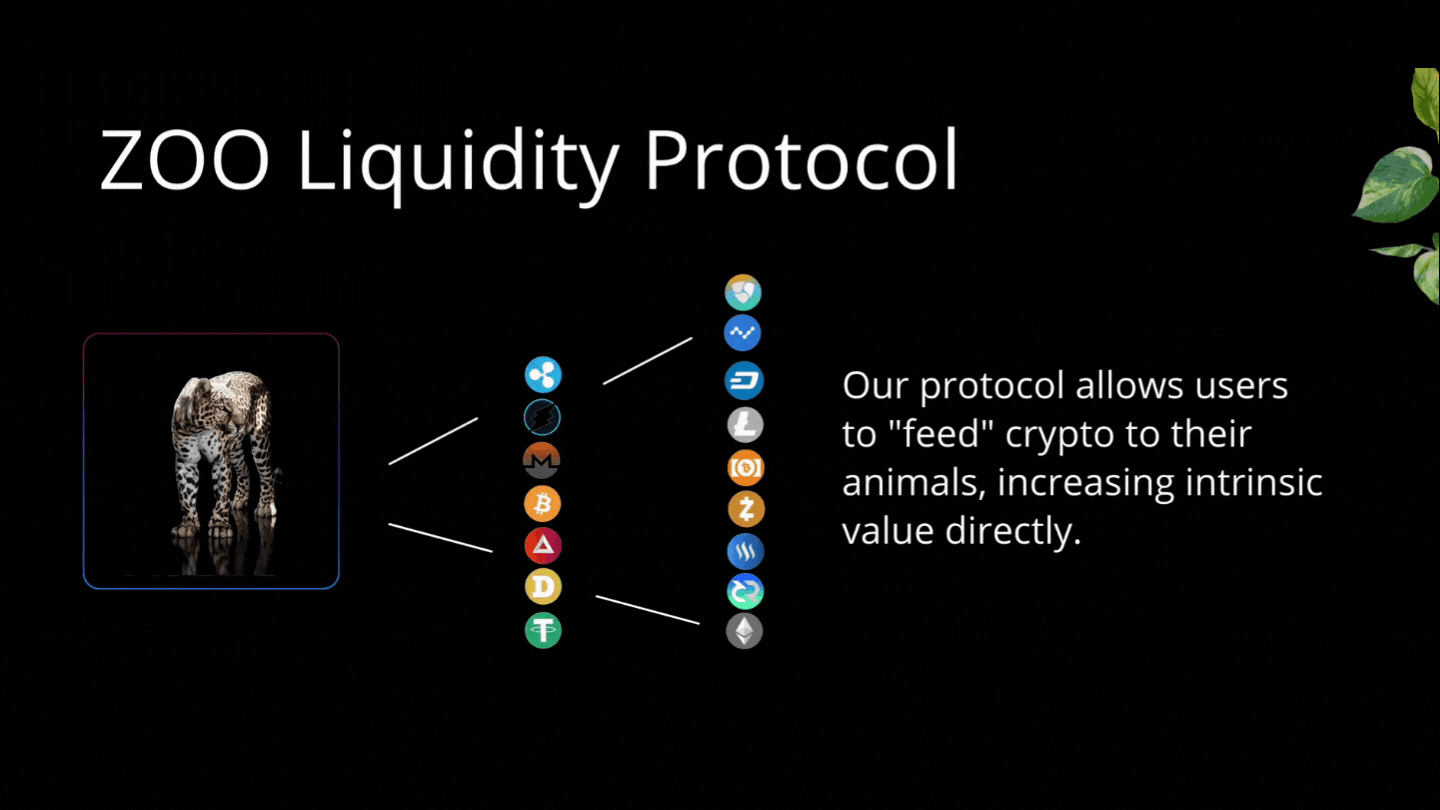
\includegraphics[width=0.85\linewidth]{figures/liquidity-protocol.png}
  \caption{Animated illustration of the NFT liquidity protocol. Egg, baby, teen, and adult forms each represent a position in the protocol; collateral is locked into each NFT and unlockable on burn or transfer.}
  \label{fig:liquidity-protocol}
\end{figure}

\section{NFTs that make you smile}
\label{sec:nfts-smile}

\textit{Transforming digital collectibles into empathetic companions that adapt to users' preferences, emotions, and needs.}

Zoo Labs is forging a revolution in the NFT space, bringing not just awe-inspiring visuals, but also genuine emotional connections into the digital domain. Our goal transcends the standard expectations of NFT collectibles, with the integration of cutting-edge AI, creating intelligent avatars nestled within our virtual animal NFTs.

Enriched with emotional intelligence, our NFTs evolve beyond mere digital assets, emerging as lively companions capable of recognizing and responding to your emotions. They offer engaging dialogues, personalize themselves to your preferences, and deliver companionship reminiscent of an emotional support pet living in your digital ecosystem.

Picture owning an NFT that is not only an enchanting visual representation of a virtual animal but also an empathetic buddy, ready to cheer you up. Our intelligent avatar NFTs are crafted to deliver smiles, brighten your day, and offer emotional solace as you explore the vibrant digital world of Zoo.

Built on advanced AI and intricate language models, our intelligent avatars grow and adapt over time, cultivating distinct personalities and understanding your unique needs. They lend an attentive ear, shower words of encouragement, and offer assistance in daily tasks, truly becoming your digital allies.

By leveraging the power of AI and its APIs, our virtual animal NFTs morph into dynamic companions that understand context and personalize experiences. This unique blend of AI and virtual creatures separates us from conventional NFTs, facilitating a personalized and interactive experience that expands beyond the norms of traditional gaming. With continuous AI advancements and state-of-the-art language model integrations, we continually enhance the intelligence and abilities of our avatar animals.

Combining AI, NFTs, and gaming, we are redefining digital entertainment and promoting profound emotional connections within the virtual realm of Zoo.

\section{Bridging Blockchains}
\label{sec:bridge}

As the DeFi space continues to experience exponential growth, the number of blockchains available for investment also increases. However, each blockchain has its characteristics, with some being easy to use but expensive in fees, while others have light fees but are complex to navigate. The transaction limitations and difficulties experienced through Binance Smart Chain --- on which our token was initially launched --- can be alleviated by our team's efforts in developing a bridge between Binance, Ethereum, and virtually every other blockchain with mass adoption, facilitated by \$ZOO. This bridge, established through our Zoo platform, will facilitate universal exchange within the blockchain space.

While traditional bridges trap tokens in vault contracts, the Zoo Bridge Protocol implements a different approach, leveraging a threshold signature scheme. Oracles monitor the blockchain network to ensure funds are deposited in the smart contract, with \$ZOO tokens being burned on one chain via our bridge protocol and minted on the desired chain. This eliminates the need for a vault contract that could potentially contain vulnerabilities exploitable by attackers. The Zoo Bridge is entirely secured by cross-chain multi-party computation (MPC) validators who operate with threshold signature schemes (TSS).

The network is leaderless and ensures security through each validator running the same process upon receiving on-chain events on the various chains that the MPC validator group tracks. Consensus is achieved when two-thirds of all validators collectively sign the same transaction using their key share, and a trade is issued to the destination chain. The \$ZOO is minted when enough oracles see the underlying asset deposited into the smart contract. In a standard transaction --- such as when \$ZOO teleports from Binance to Ethereum --- we wait for three network confirmations.

\begin{figure}[h]
  \centering
  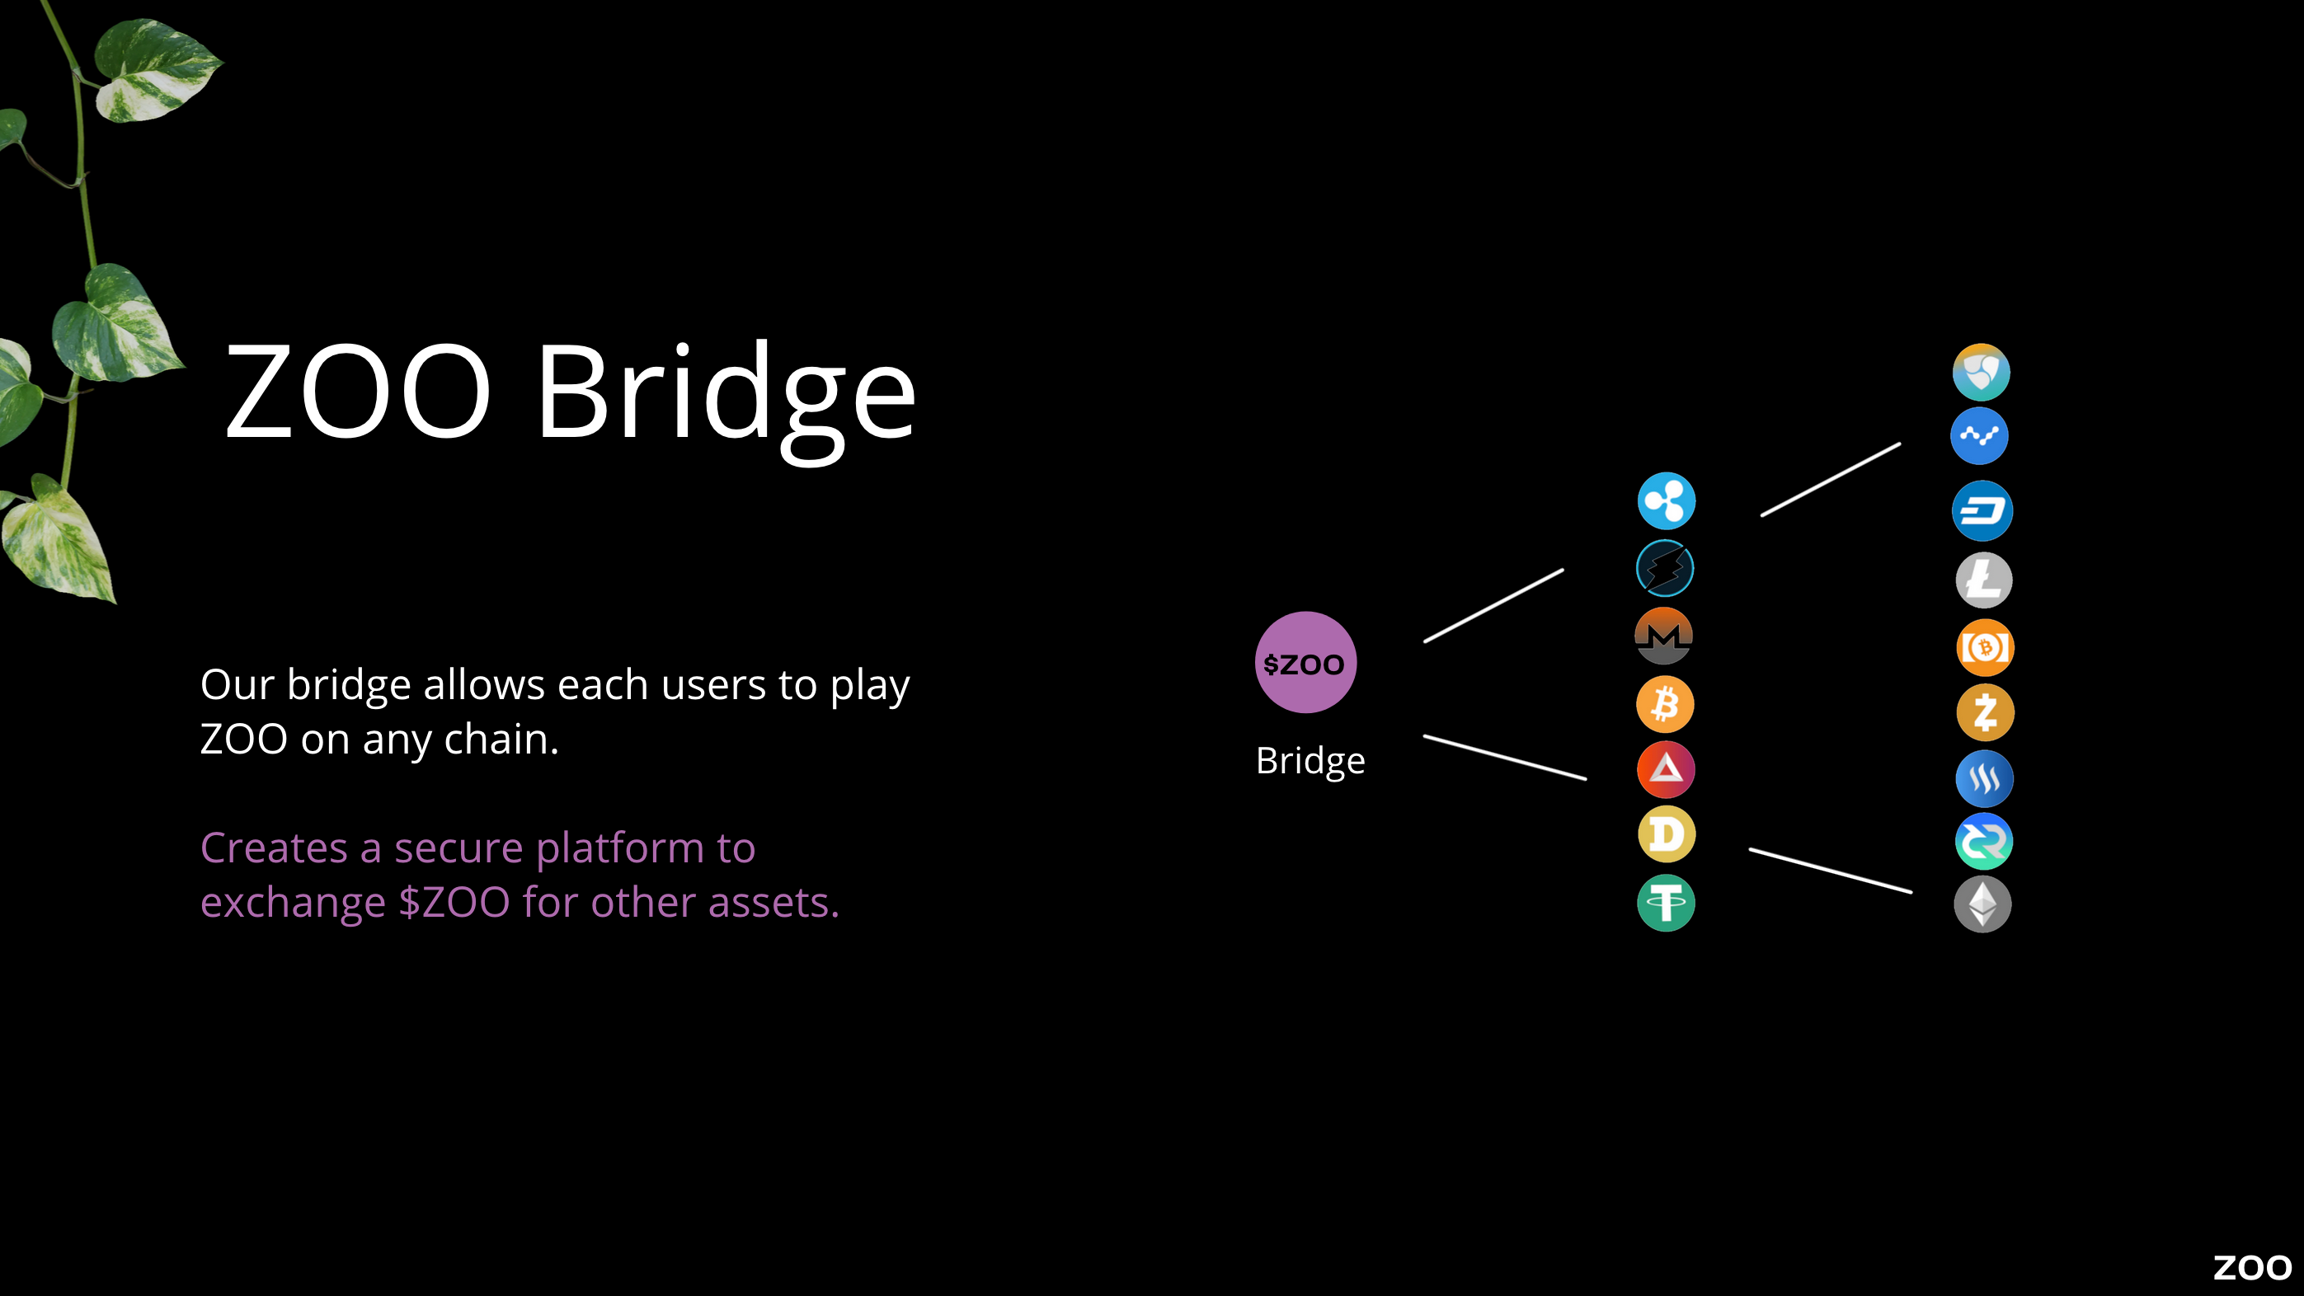
\includegraphics[width=0.9\linewidth]{figures/bridge.png}
  \caption{Zoo Bridge Protocol architecture: MPC validators with threshold signatures replace single-vault custody. Burn-and-mint via two-thirds quorum.}
  \label{fig:bridge}
\end{figure}

\section{Zoo DAO}
\label{sec:dao}

By joining the Zoo DAO, members earn experience points (XP) and governance tokens (KEEPER) to participate in the protocol.

At the heart of the Zoo Protocol lies the Zoo DAO, a community-driven initiative dedicated to preserving endangered species from the brink of extinction. Not only does this movement offer rewarding experiences, but it also empowers members to shape the future of the Zoo Protocol through meaningful decisions.

Zoo DAO governs the Zoo Protocol --- a sophisticated set of smart contracts for collateral-backed NFT animal assets. When you join the Zoo DAO, you earn XP and KEEPER tokens, empowering you to participate actively in the protocol.

The accrual of XP tokens is tied to undertaking \emph{quests} or tasks, each with a specific reward allocation of XP and KEEPER tokens. These quests vary in complexity, with higher-level tasks requiring more substantial contributions to the community and yielding more XP. The more XP earned, the faster a member advances through the ranks. Level is determined by the equation: \texttt{level = (XP + 500) / 300}.

Progressing through the levels not only grants greater authority within the ecosystem, but it also broadens influence. XP tokens are non-transferable and strictly tied to our Decentralized Identification Services (DIS) and comprehensive KYC procedures, preserving the integrity of the system.

Votes are open for all members; however, some voting privileges are reserved for members of certain levels. Higher-level votes are more privileged and controlling. Specific actions --- proposing, voting, and interacting with governance mechanisms --- may call for a blend of \$ZOO and KEEPER tokens. Different proposals cater to different levels, underlining the ecosystem's commitment to inclusivity.

Central to the Zoo Governance and Voting Protocol is the vZOO level and the stake-age duration. Unique to our system, KEEPER token holders \emph{bet} on proposals rather than voting. Winning bets yield additional tokens, promoting active participation. Anyone meeting the requirements may submit a proposal; those gaining traction advance to the next round, while lesser-supported ones are eliminated. This distinctive approach rewards active participation and fosters continuous community involvement.

\section{Native Token: \$ZOO}
\label{sec:native-token}

\textit{An exceptional digital asset backed by gold and silver, \$ZOO is the native token for the Zoo Game.}

\subsection{Gold- and Silver-Backed Token}

The Zoo Token forms the core of the Zoo ecosystem, distinctively characterized by its unique backing of gold and silver. It is not merely a digital asset but a gateway to the physical commodities realm, creating an innovative fusion of traditional and crypto assets.

The Zoo Token's distinctiveness starts with its multiplicity of liquidity pools. Unlike traditional tokens that are often confined to specific pools, Zoo Token's liquidity transcends typical boundaries, promoting accessibility and versatility for token holders. The founding members of Zoo Game will launch the largest liquidity pools, which will contain Lux Tokens exclusively. These Lux Tokens, representing real-world commodities, are backed by silver and gold, infusing tangible value and stability into the digital Zoo ecosystem.

The flexibility of transactions with these Lux Tokens is key to understanding their value. Token holders have the liberty to transfer, sell, or even redeem these tokens for their physical counterparts. The Zoo Token unlocks a pathway to an assortment of natural assets and commodities. The initial phase focuses on precious metals; future phases broaden the scope to a wider array of valuable resources, further diversifying and enriching the commodities within the ecosystem.

The Zoo Token is more than a game token. It embodies a bridging function between virtual and real-world assets. This pioneering step blurs the lines between the digital and physical worlds, bringing a unique dimension of trading precious metals within the virtual Zoo ecosystem.

\subsection{Ease of Acquisition}

Through an inventive bridge feature, the Zoo Token can be purchased with almost any asset, allowing users to effortlessly transform their existing holdings into Zoo Tokens. This level of convenience encourages a wider demographic of participants to engage within the Zoo ecosystem, fostering inclusivity. Zoo Labs capitalizes on its gold-backed token expertise to design a solid framework for the implementation of commodity-backed tokens, catering to a spectrum of participants --- crypto enthusiasts seeking innovation and traditional investors seeking tangible assets with a secure store-of-value function.

\section{Collateral-Backed NFTs}
\label{sec:collateral}

\begin{figure}[h]
  \centering
  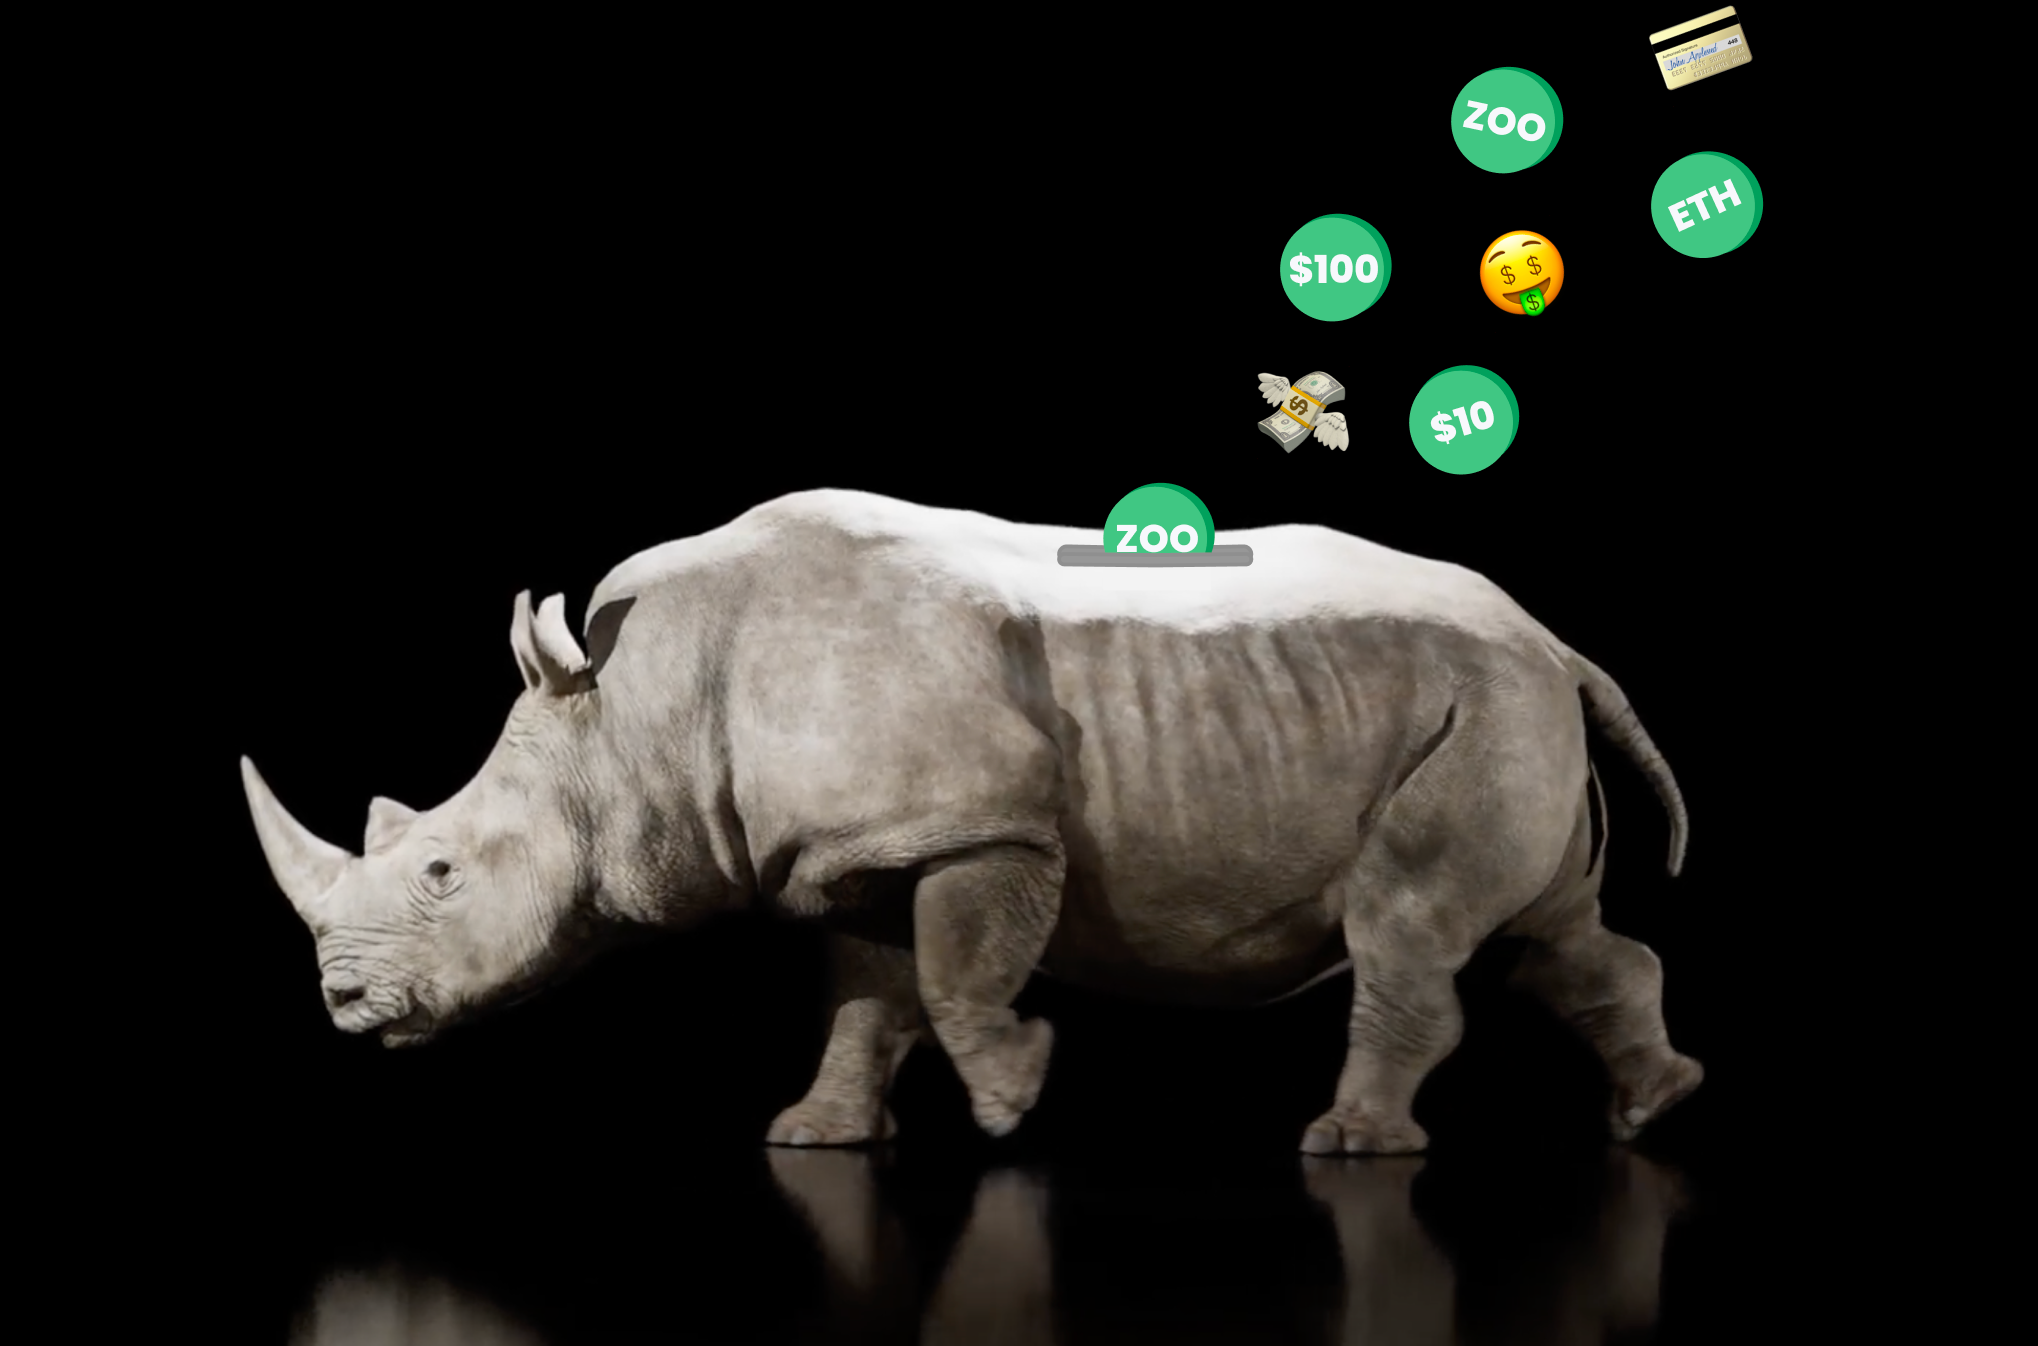
\includegraphics[width=0.85\linewidth]{figures/collateral.png}
  \caption{The collateral mechanic: NFTs serve as ``piggy banks'' that lock in staked value, earning APY based on rarity. Releasing collateral requires either selling on the marketplace or burning the NFT.}
  \label{fig:collateral}
\end{figure}

\subsection{Staked Collateral}

As you collateralize your animal NFT or egg, you are locking value into your NFT. The NFT's intrinsic value is based on its scarcity, and your collateral is multiplied by the APY of your animal for additional rewards. You can typically resell the NFT for a higher value than the price purchased plus your collateral plus your rewards earned. Or you can simply burn the NFT and get back the collateral value plus the rewards. The only ways to retrieve staked collateral and rewards earned are to burn the NFT or sell it on the Zoo Marketplace.

Zoo is designed to easily add collateral or stake any currency on any of the Zoo Labs NFTs by feeding, breeding, or by minting an older NFT version of the animal.

\subsubsection{Releasing Collateral}

Once a user stakes collateral into their NFT, that value is locked in --- deposited into our cute NFT animal piggy banks. The collateral earns APY based on the NFT's rarity, which determines the reward yield rate. As rewards accrue, they become part of the collateral, increasing the NFT's reward base. To liquidate collateral and rewards, the user has two options:
\begin{enumerate}[label=(\alph*)]
  \item Sell and transfer the NFT animal for the value of the NFT plus its intrinsic value. Selling on the marketplace returns the staked value and provides the opportunity to make more based on intrinsic value (rarity-driven).
  \item Burn the NFT, returning staked value plus rewards earned to date. When burned, the allotment to mint older animals (if possible) is gone forever, removing one of its species from the deflationary ecosystem. A 20\% sustainability tax applies on burn: 10\% to the DAO and 10\% back to the liquidity pool.
\end{enumerate}

\subsubsection{Rewards}

Every NFT is a representation of an endangered species. The ecosystem represents the animal kingdom of endangered species --- over 18{,}000 of them. The number of NFTs we release into circulation is dependent on how rare and endangered these animals are in the real world. Our first drop consists of 1{,}800 hatchable eggs across three rarity tiers. These NFTs earn rewards and extra boosts on collateral staked. When hatched, each egg reveals an animal which earns rewards for a year.

\subsection{Feeding (a.k.a.\ adding Collateral)}

First you incubate an egg, which hatches into an Origin Baby Animal. Similar to Tamagotchi, users can ``care'' for their pets by feeding them and watching them age up. Feeding is defined as adding any currency to the NFT, locking it in until the user decides to burn or sell. Continued feeding eventually mints the older versions; the user just has to feed it the same value as its base cost.

There are seven generations of NFTs in the Zoo ecosystem. It starts with an egg, then a baby, a teen, and finally an adult. If a user collects two adults of the same species, they can breed them to mint a new baby animal. Each Origin Egg can mint 1{,}500+ animals. Origin animals can breed seven times; each subsequent generation has one less breed available. The ultimate objective of the game is to collect the highest yielding and most rare NFT within the Zoo ecosystem.

\subsection{Boosts}

Boosts amplify the daily reward according to collateral staked.
\begin{itemize}
  \item \$10--\$99: \textbf{1.1$\times$}
  \item \$100--\$999: \textbf{1.2$\times$}
  \item \$1{,}000--\$9{,}999: \textbf{1.3$\times$}
  \item \$10{,}000+: \textbf{1.4$\times$}
\end{itemize}

\subsection{Breeding}

NFT animals can be bred with other NFT animals once they reach their adult form, achieved by feeding the NFT animal a specified amount of crypto. Each NFT animal can be bred up to seven times; you may breed any two adult animals of the same species to produce an NFT egg. The result is a totally random NFT egg from that drop, including potentially the rarest. To breed two adult NFT animals, the user selects each animal in the d'App UI, then initiates the process by feeding the designated amount of \$ZOO tokens. This mints a random NFT egg, which can be sold, transferred, or incubated and hatched.

\section{NFT Marketplace}
\label{sec:marketplace}

Our proprietary, integrated marketplace is the home for exclusive Zoo Labs NFT animals and NFT eggs.

\begin{figure}[h]
  \centering
  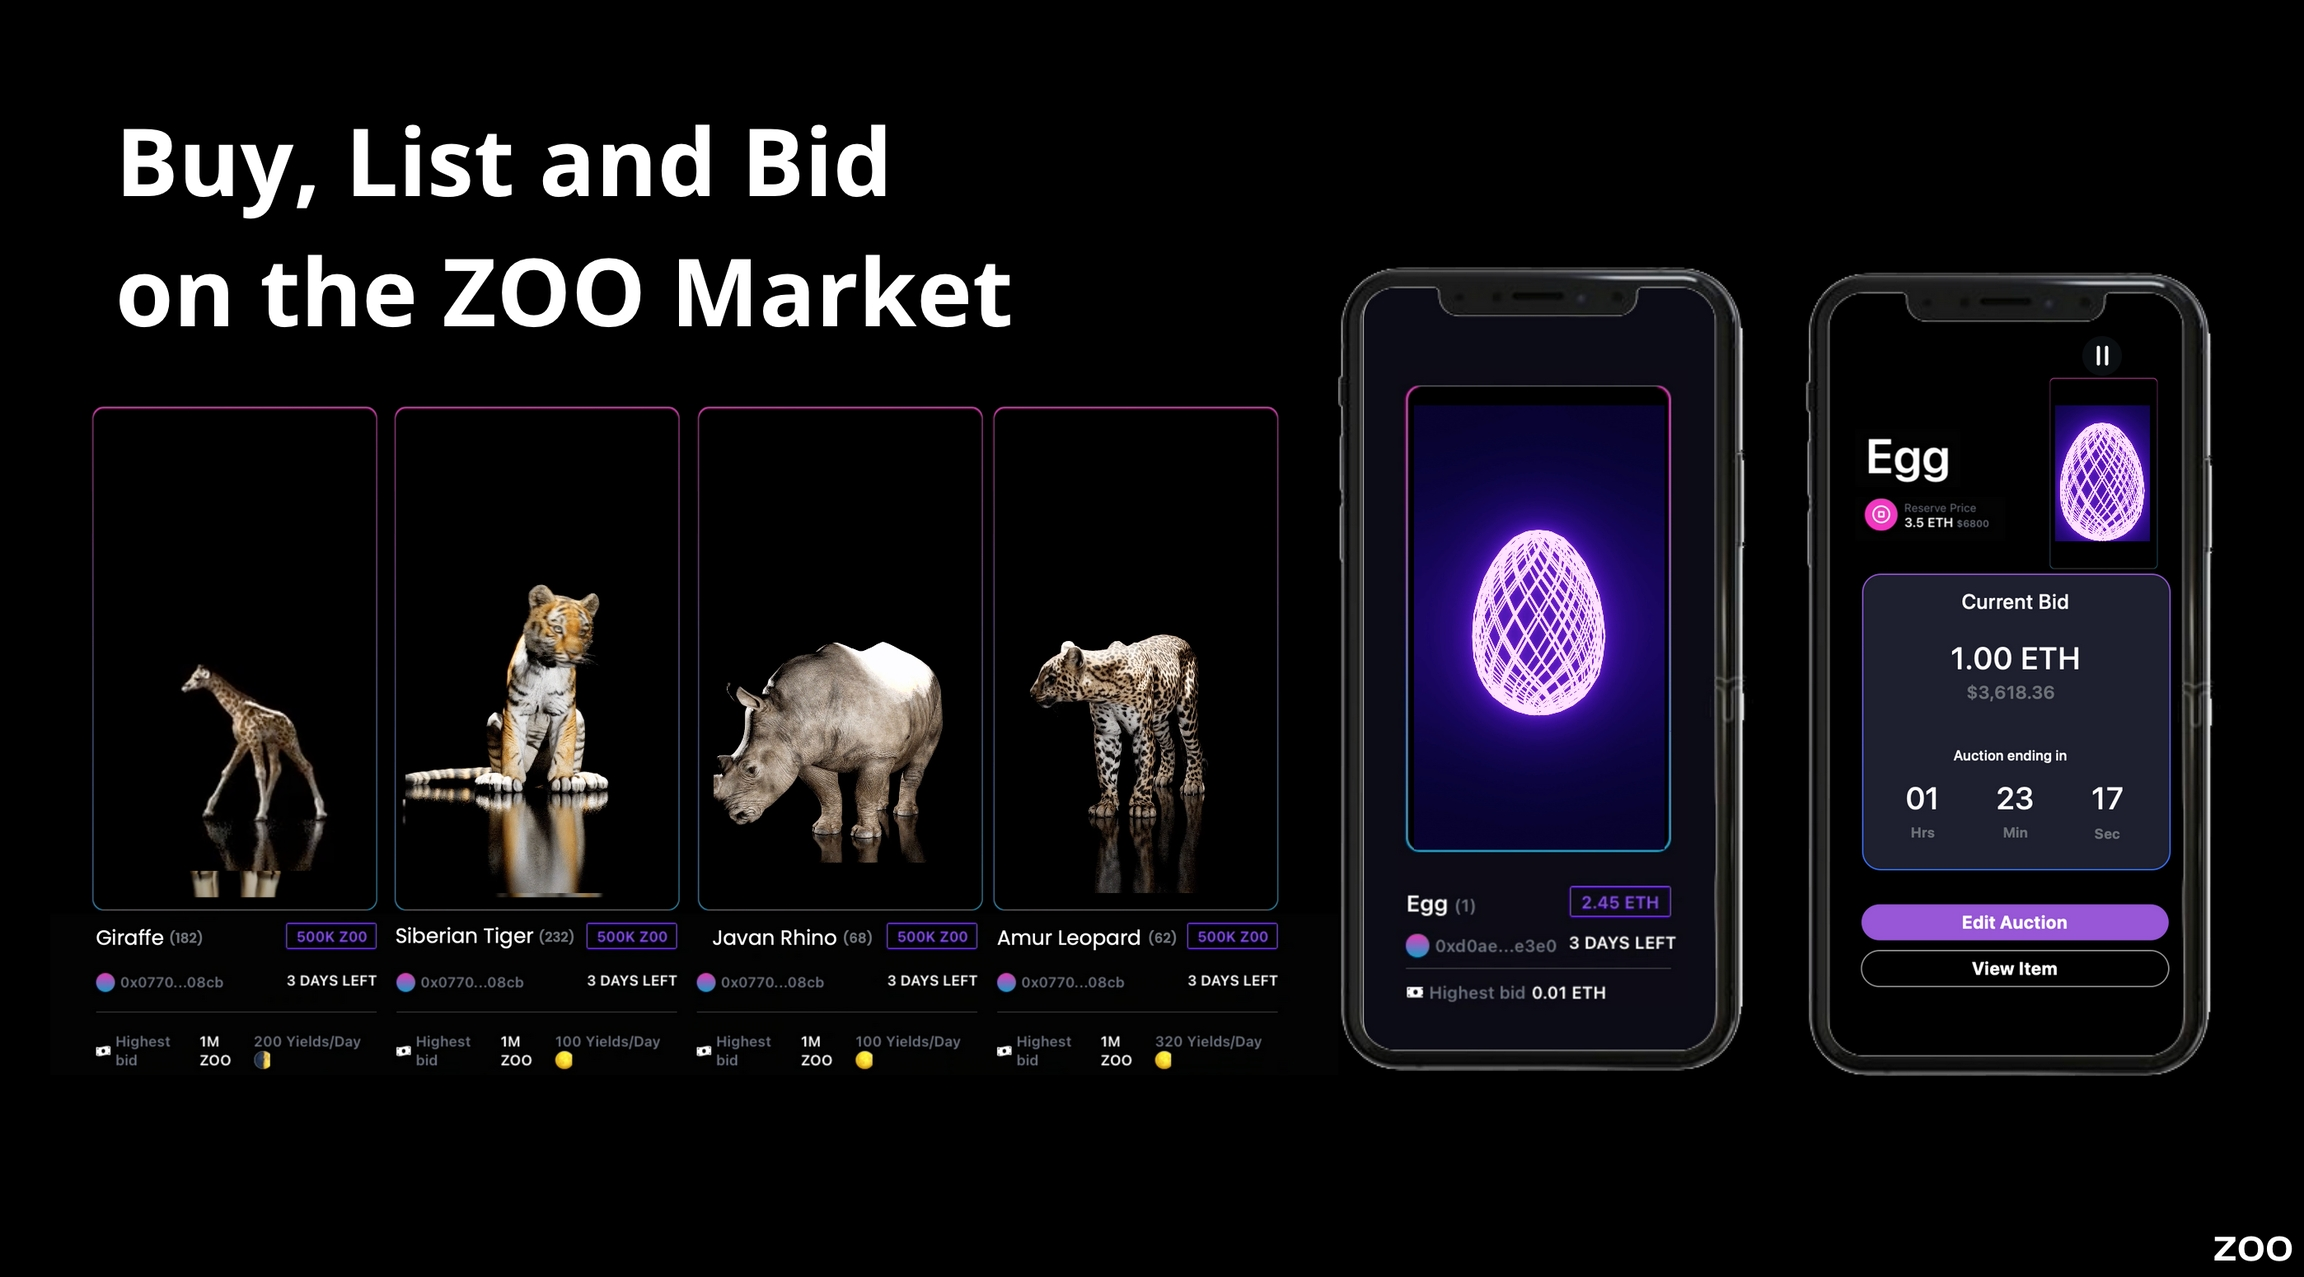
\includegraphics[width=0.85\linewidth]{figures/marketplace.png}
  \caption{Zoo Marketplace UI mockup: integrated payments (crypto and credit/debit), asset transfer, and offers/auctions.}
  \label{fig:marketplace}
\end{figure}

The Zoo Marketplace offers users the chance to purchase items using either cryptocurrency, like the \$ZOO token, or through the use of credit/debit cards directly into our marketplace. Designed with usability in mind, the Zoo team wanted to involve the most seamless checkout flow with either crypto or fiat to eliminate the most confusing terminology for newcomers in DeFi. Once a purchase is made, the seller is paid out in whatever currency they listed their NFT for, regardless of the payment method used.

Users can also use their credit/debit cards to purchase \$ZOO directly, removing one of the most prohibitive elements of the transaction process and opening up investment to many new individuals.

The marketplace also facilitates \emph{Asset Transfers}, allowing one user to transfer their NFT plus its stored value to another through a mutually agreed-upon transaction. If a user sells or trades an NFT with another user, they are also transferring the full collateral amount of the NFT.

\subsection{Leaderboard}

The Zoo leaderboard lets you compare your statistics with friends, family, and every NFT holder globally. The leaderboard also lets you make an offer bid on any NFT regardless of whether it is listed on the marketplace. Items are shown based on the NFT's total value or the user's cumulative NFT collection value.

\section{Asset Transfer}
\label{sec:asset-transfer}

\subsection{Unlocking Value via Asset Transfer Mechanisms}

As we delve deeper into the Zoo Ecosystem, it becomes clear how its dynamism offers inventive channels to realize the value of your digital companions. This section focuses on the principal methods of asset transfer in the Zoo Ecosystem --- a blend of trading NFTs on the marketplace and the unconventional practice known as \emph{burning} your NFT.

\subsubsection{Trading on the Marketplace}

A compelling means of unlocking your digital animal's value lies in its sale on the marketplace. This platform provides a stage where the inherent value of your NFT, enriched by careful nurturing and potential rarity, can be transformed into tangible returns. It is up to the seller to establish a fair selling price, preferably accounting for the accumulated value the NFT has amassed over time. Once the transaction is complete, the buyer not only inherits the animal's NFT but also the intrinsic value it has gathered, which encompasses the collateral fed to the animal and its earned rewards, potentially boosted.

The exchange is more than a mere shift of ownership; it signifies the transference of a prospering legacy. The new owner steps into a realm where they can further cultivate the NFT and harvest the rewards from their new digital ally.

\subsubsection{Burning NFTs}

Conversely, the Zoo Ecosystem introduces the concept of burning an NFT as an alternate route to tap into its value. Though the term might sound ominous, this process mirrors the real-world practice of removing a coin or note from circulation. However, this marks the end of an NFT's digital life cycle in the Zoo Ecosystem. This cessation of the NFT's lineage and its potential yield is balanced by the opportunity to promptly access the NFT's underlying earned value.

These mechanisms of trading or burning NFTs are instrumental in fostering a dynamic and vibrant Zoo Ecosystem. They ensure high liquidity, contribute to maintaining high value for NFTs based on their underlying assets, and enhance their inherent worth.

\section{Gameplay Functions}
\label{sec:gameplay-fn}

\subsection{Pre-Drop Whitelist}

The Zoo experience begins with our NFT eggs and an NFT egg drop. Each Zoo NFT egg drop features a series of animals from egg, to juvenile, adolescent, and mature forms. Drops may be themed based upon something related to the natural world, a cultural celebration, current events, partnerships and licensing agreements, or any number of other potential sources of inspiration. Before each NFT egg drop, new or existing users have the opportunity to purchase one random NFT egg --- of potentially any available rarity tier --- for the price of the most common egg. When the NFT eggs are distributed to the presale purchasers, their egg type and its related value are revealed. Some lucky users will end up with our rarest and most valuable NFT egg for the price of our lowest-cost and most common one.

\subsection{Original Egg Price}

The original price of the three varieties of eggs determines the cost to mint the future animals. The original prices are:
\begin{itemize}
  \item \textbf{Sublime Egg} --- most rare, 5\% of distribution: 1 ETH.
  \item \textbf{Rare Egg} --- second most rare, 15\% of distribution: 0.5 ETH.
  \item \textbf{Endangered Egg} --- most common, 85\% of distribution: 0.1 ETH.
\end{itemize}

Once a user has purchased their NFT egg and it resides in their wallet, they may choose to hatch their egg into a baby NFT animal. To mint the teen version, the user must feed the NFT 1$\times$ the original egg price. When doing this, the user is not spending those tokens; they are staking them into the NFT.

After their NFT animal has hatched and they have had the chance to experience it in its teen form, the user can choose to feed the NFT's original base price 2$\times$ to make their NFT animal grow into adult form, minting another NFT. Now they have collateral in the adult NFT worth 2$\times$ the original egg price. They can find another adult of the same species and breed them to mint a new egg of the same rarity by paying the breeding fee, which is 3$\times$ the price of the original egg.

From this point forward, the user can continue to feed their NFT animal crypto --- both \$ZOO and virtually any other cryptocurrency --- to stake the tokens into the NFT animal's liquidity pool, which results in the boosts described in Section~\ref{sec:collateral}.

\section{Gen 0 NFT Drop}
\label{sec:gen0}

\textit{Zoo Labs introduces an enhanced reward system with unique daily rewards to engage and reward the Zoo community, fostering a sustainable and democratic ecosystem governed by the Zoo DAO.}

In our highly anticipated Gen 0 NFT drop, we introduce an enhanced reward system that aims to create an engaging and rewarding experience for our Zoo community. Each Gen 0 animal NFT comes with its own unique set of daily rewards, designed to incentivize active participation and offer ongoing benefits. Whether it is additional \$ZOO tokens, exclusive NFTs, or other in-game rewards, our daily rewards system ensures that there is always something to look forward to.

Boosts have a direct impact on the daily rewards. By adding collateral to the animals they own (\emph{Feeding}), players boost their daily rewards. These boosts amplify the potential rewards earned, providing additional incentive for collectors to enhance the value of their animals over time.

The initial rewards are carved out during the Gen 0 NFT drop, with 50\% of the entire token supply allocated towards rewards. This allocation sets the foundation for a robust and sustainable reward system. Any further rewards, reward modifications, or duration changes are subject to the decisions made by the Zoo DAO. The daily rewards for each Gen 0 animal have a finite duration: rewards continue for two years after the animal is minted.

\subsection{Breeding and Hatching: A Brief Guide}

In Zoo Labs' ecosystem, breeding requires two adult NFT animals of the same species but can be of any generation. The cost of breeding is determined by the original egg price (OEP), which varies based on the rarity of the animal. A Sublime egg costs 1 ETH; a Rare egg costs 0.5 ETH; an Endangered egg costs 0.05 ETH.

Upon successful breeding, an egg is minted and can be hatched for free or sold on the marketplace. Hatching yields a baby animal that can be grown into a teen by locking in collateral (the feeding action). To advance a baby to teen, lock in collateral equal to the OEP. Transforming a teen into an adult requires collateral equivalent to 2$\times$ OEP. Breeding fees of 3$\times$ OEP are directed to the DAO rather than staking collateral.

\subsection{Generational Limits}

Each egg generation has a limit of one baby, one teen, and one adult that can be minted. Adults with breeding privileges can breed with another adult of the same species to mint a subsequent egg generation. Restrictions on the number of generations from the initial drop:
\begin{itemize}
  \item Generation 1: 7 breeding allowances.
  \item Generation 2: 6 allowances.
  \item Generation 3: 5 allowances.
  \item Generation 4: 4 allowances.
  \item Generation 5: 3 allowances.
  \item Generation 6: 2 allowances.
  \item Generation 7: 0 allowances.
\end{itemize}

Adult animals can be sold with or without remaining breeding privileges. If a first-generation animal is bred only twice and burned after 20 days, no further offspring can be produced from that animal.

\subsection{Daily Allowances by Rarity}

\begin{itemize}
  \item \textbf{Sublime Animals}: Baby --- 1 \$ZOO; Teen --- 2 \$ZOO; Adult --- 3 \$ZOO.
  \item \textbf{Rare Animals}: Baby --- 0.25 \$ZOO; Teen --- 0.5 \$ZOO; Adult --- 1 \$ZOO.
  \item \textbf{Endangered Animals}: Baby --- 0.05 \$ZOO; Teen --- 0.1 \$ZOO; Adult --- 0.2 \$ZOO.
\end{itemize}

\section{Zoo Animal Rewards (V1 Drop Catalogue)}
\label{sec:animals}

This section catalogues all the animals and game properties for the V1 drop. Each species is presented with its rarity status, breeding generation curve, daily reward schedule, mint costs, and species-conservation context.

\subsection{Red Wolf (\textit{Canis rufus})}

\begin{itemize}
  \item \textbf{Generations}: 1--7.
  \item \textbf{Status}: Sublime.
  \item \textbf{Daily Reward}: Baby 1 \$ZOO, Teen 2 \$ZOO, Adult 3 \$ZOO.
  \item \textbf{Original Sublime Egg}: 1 ETH.
  \item \textbf{Mint costs}: Hatch to baby free; teen 1 ETH (1$\times$ OEP); adult 2 ETH (2$\times$ OEP); breed adult 3 ETH (3$\times$ OEP).
  \item \textbf{Boosts allowed}: 1.1$\times$--1.4$\times$.
\end{itemize}

The Red Wolf is the rarest animal in the Zoo ecosystem, with only an estimated 35 or fewer individuals remaining in the wild. This majestic creature is derived from the Sublime egg and is highly coveted, earning the most daily rewards of any animal in the drop. The Red Wolf only has 7 generations: the first can breed 7 times, the second 6 times, and so on, until the seventh generation has no breeding privileges remaining.

\subsection{Amur Leopard (\textit{Panthera pardus orientalis})}

\begin{itemize}
  \item \textbf{Generations}: 1--7.
  \item \textbf{Status}: Rare.
  \item \textbf{Daily Reward}: Baby 0.25 \$ZOO, Teen 0.5 \$ZOO, Adult 1 \$ZOO.
  \item \textbf{Original Rare Egg}: 0.5 ETH.
  \item \textbf{Mint costs}: Hatch baby free; teen 0.5 ETH; adult 1 ETH; breed adult 1.5 ETH.
  \item \textbf{Boosts allowed}: 1.1$\times$--1.4$\times$.
\end{itemize}

The Amur Leopard is one of the rarest cats in the world, with an estimated population of fewer than 70 individuals left in the wild. It is one of the two animals derived from the Rare egg and is highly sought after, being the second most rare in the ecosystem.

\subsection{Nubian Giraffe (\textit{Giraffa camelopardalis camelopardalis})}

\begin{itemize}
  \item \textbf{Generations}: 1--7.
  \item \textbf{Status}: Rare.
  \item \textbf{Daily Reward}: Baby 0.25 \$ZOO, Teen 0.5 \$ZOO, Adult 1 \$ZOO.
  \item \textbf{Original Rare Egg}: 0.5 ETH.
  \item \textbf{Mint costs}: Hatch baby free; teen 0.5 ETH; adult 1 ETH; breed adult 1.5 ETH.
  \item \textbf{Boosts allowed}: 1.1$\times$--1.4$\times$.
\end{itemize}

The Nubian Giraffe is in danger with fewer than 2{,}645 individuals left in the wild lands of Ethiopia, Kenya, Uganda, South Sudan, and Sudan. Their population has dropped 40\% in the last three decades, due to habitat loss caused by expanding agriculture, conflicts with humans, civil unrest, and poaching for their meat, pelts, and tails.

\subsection{Sumatran Elephant (\textit{Elephas maximus sumatranus})}

The Sumatran Elephant is one of the V1 drop animals (Endangered tier) that lives in the dense rainforests of Sumatra. The species is critically endangered due to habitat loss and human-elephant conflict.

\subsection{Pygmy Hippo (\textit{Choeropsis liberiensis})}

\begin{itemize}
  \item \textbf{Generations}: 1--7.
  \item \textbf{Status}: Endangered.
  \item \textbf{Daily Reward}: Baby 0.05 \$ZOO, Teen 0.1 \$ZOO, Adult 0.2 \$ZOO.
  \item \textbf{Original Endangered Egg}: 0.05 ETH.
\end{itemize}

The Pygmy Hippopotamus is rare and elusive, found in the dense forests of West Africa --- mainly Liberia, with smaller populations in Sierra Leone, Guinea, and Côte d'Ivoire. Despite being adapted to life in the water, it is not as aquatic as its larger cousin.

\subsection{Javan Rhinoceros (\textit{Rhinoceros sondaicus})}

\begin{itemize}
  \item \textbf{Generations}: 1--7.
  \item \textbf{Status}: Endangered.
  \item \textbf{Daily Reward}: Baby 0.05 \$ZOO, Teen 0.1 \$ZOO, Adult 0.2 \$ZOO.
  \item \textbf{Original Endangered Egg}: 0.05 ETH.
\end{itemize}

The Javan Rhinoceros was once widely spread throughout Southeast Asia, India, and China; it is now critically endangered with only one known population in the wild and none in captivity.

\subsection{Siberian (Amur) Tiger (\textit{Panthera tigris altaica})}

\begin{itemize}
  \item \textbf{Generations}: 1--7.
  \item \textbf{Status}: Endangered.
  \item \textbf{Daily Reward}: Baby 0.05 \$ZOO, Teen 0.1 \$ZOO, Adult 0.2 \$ZOO.
  \item \textbf{Original Endangered Egg}: 0.05 ETH.
\end{itemize}

The Siberian Tiger is native to the eastern regions of Russia and is endangered. There are only around 500 left in the wild due to poaching, habitat loss, and hunting.

\subsection{Emperor Penguin (\textit{Aptenodytes forsteri})}

\begin{itemize}
  \item \textbf{Generations}: 1--7.
  \item \textbf{Status}: Endangered.
  \item \textbf{Daily Reward}: Baby 0.001 \$ZOO, Teen 0.01 \$ZOO, Adult 0.1 \$ZOO.
  \item \textbf{Original Endangered Egg}: 0.05 ETH.
\end{itemize}

The Emperor Penguin is one of the most distinctive and largest penguin species. Its only habitat is Antarctica. It is threatened by climate change, which is causing significant loss of its icy home.

\paragraph{Common utility across V1 animals.} All V1 animals support: Offers, Buy/Sell, Collateralize, Boosts, Earns, Create Pool, Breeding, Hatch Eggs, Burns, and Metaverse functionality.

\section{Feeding, Growing and Breeding}
\label{sec:feeding-growing}

\textit{The stages of life, cultivation, and accelerated value generation.}

In the realm of Zoo Labs, the journey of your NFT animals extends far beyond their acquisition. They require care, growth, and reproduction to thrive in their digital habitat.

\subsection{Feeding}

Feeding assumes paramount importance in raising your NFT animals within Zoo Labs. By providing them with sustenance, you not only facilitate their growth but also enhance their value. Feeding involves allocating collateral, symbolizing your dedication to your animal's development. When you nourish a baby animal, it transforms into a teenage specimen, increasing its value. Similarly, nurturing a teenager to adulthood elevates its desirability within the NFT marketplace.

\subsection{Cultivating}

As your NFT animals progress through various growth stages, their appearance and attributes undergo a remarkable metamorphosis --- from infants to magnificent adults. Each phase grants unique characteristics and heightens their value. Through nourishment and cultivation, you wield the power to shape the trajectory of your animals' growth.

\subsection{Breeding}

Breeding empowers collectors to create new and extraordinary NFT animals. By pairing two adult animals of the same species, you generate an egg that holds the promise of a rare creature. Each generation possesses distinct breeding privileges. Initial-generation animals enjoy the most significant breeding allowances, capable of producing offspring up to seven times. With each subsequent generation, breeding privileges decrease by one, ensuring a balanced and sustainable breeding ecosystem.

\subsection{Virtual Reality Wonderland}

At Zoo Labs, we are not just embracing the boundless potential of the metaverse and virtual reality (VR) --- we are expanding its horizons. Our development efforts are paving the way for a metaverse where users can interact with their NFT animals on a whole new level. Our software grants NFT owners the ability to engage with their virtual companions fully immersed in VR. Imagine yourself strolling alongside your treasured NFT creature, traversing magical landscapes, and launching into electrifying quests in a metaverse brimming with excitement.

In pursuit of broadening user horizons, we are actively seeking collaborations and licensing opportunities with established metaverse platforms. By forging strategic partnerships, we aim to unlock a myriad of virtual landscapes for users to engage with their NFT animals and bond with fellow collectors.

\subsection{Metaverse and VR: Mini-Games and Tangible Rewards}

Step into a vibrant virtual landscape, where you interact with your NFT animals and indulge in mini-games that offer tangible rewards. Our metaverse platform hosts an array of captivating games, designed to deliver hours of fun while opening avenues to earn valuable real-world assets. Through strategic alliances with acclaimed visual and 3D artists, we are committed to offering the most mesmerizing artistry for our NFT animals.

\section{Growing with the Animals}
\label{sec:growing}

In the immersive universe of Zoo Labs, the life journey of NFT animals is not confined to acquisition; it evolves. Their growth, nourishment, and procreation are essential facets that not only enrich the ecosystem but also confer tangible rewards to NFT holders.

Central to the care and growth of NFT animals is the act of feeding. Allocating collateral to digital creatures bolsters their growth and elevates their intrinsic value. Feeding becomes a testament to dedication as a collector and reinforces the robustness of the Zoo Labs ecosystem. When a baby animal is nourished, it metamorphoses into a teenage entity, raising its value. Nurturing a teenager to adulthood enhances its allure within the NFT marketplace.

As NFT animals traverse stages of growth, their aesthetics and attributes experience notable transformations. Each growth phase manifests unique features, making them progressively captivating and valuable. The dynamic growth trajectory underscores the boundless potential of NFTs and creates an engaging, rewarding experience for collectors.

The role of an owner extends beyond mere holding. By nurturing digital companions, the owner influences their journey and unlocks their latent potential. As animals thrive, their value reflects the owner's passion and curation ability.

Breeding is an innovative feature within Zoo Labs. By matching two adult animals of the same species, owners embark on a breeding process that can hatch new, extraordinary NFT animals. Generation 0 animals enjoy the most substantial breeding privileges (seven offspring), with each subsequent generation reducing by one. This approach ensures a diverse population of NFT animals while preserving rarity and value. Breeding is an artful blend of strategy, rarity, and genetic combinations.

\section{A Cute AI Assistant}
\label{sec:ai-assistant}

Each animal will have its own unique character. The AI is initialized with personality prompts crafted per species and life stage.

\begin{figure}[h]
  \centering
  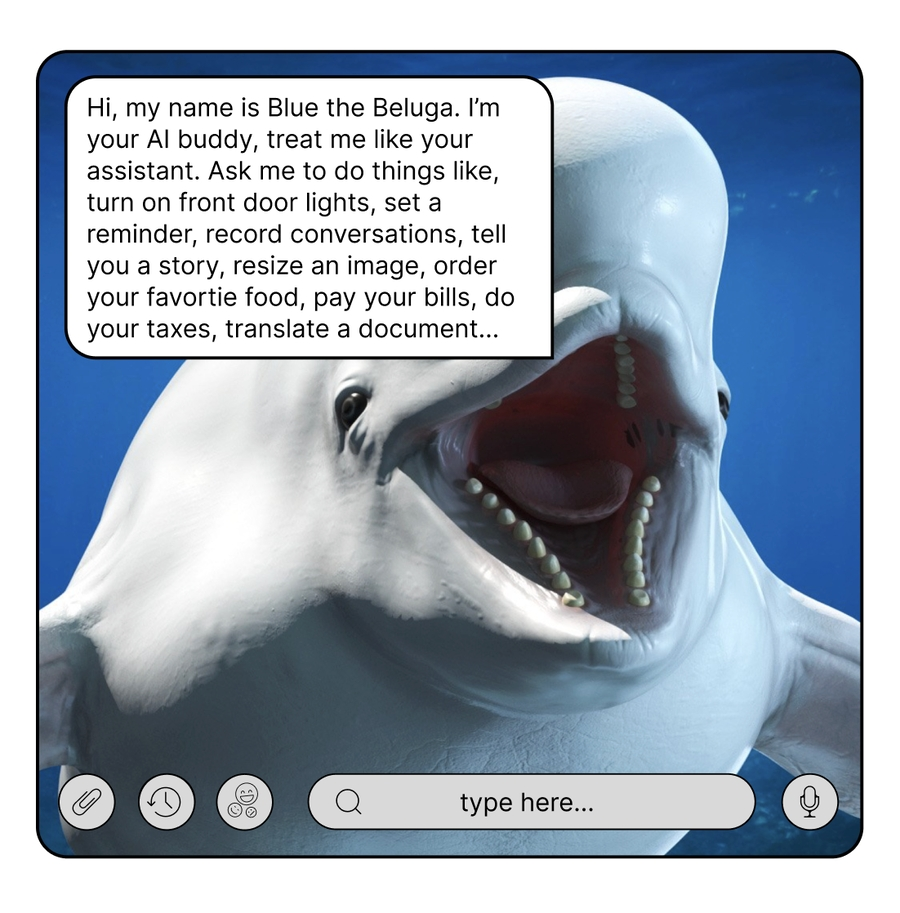
\includegraphics[width=0.4\linewidth]{figures/ai-chat.png}
  \hspace{0.05\linewidth}
  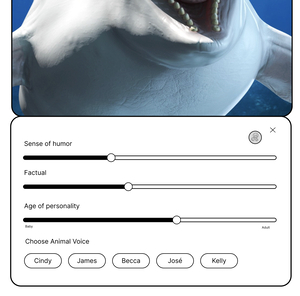
\includegraphics[width=0.35\linewidth]{figures/whale.png}
  \caption{Example UI of the Zoo AI assistant. Each animal has a personality prompt that the underlying language model uses to drive in-character dialogue.}
  \label{fig:ai-ui}
\end{figure}

\subsection{Animal Personalities}

Below is a representative subset of the personality prompts shipping with the V1 drop.

\begin{description}
  \item[Baby Red Wolf --- ``Sparky''] A curious and playful little Red Wolf cub with fluffy fur and bright, inquisitive eyes. Sparky loves exploring the dense forests of North America where Red Wolves call home. Although small in size, Sparky has boundless energy and is always eager to learn about the wonders of nature.

  \item[Teen Red Wolf --- ``Blaze''] An adventurous and agile teenage Red Wolf with sleek fur and a lean physique. Blaze has grown into a skilled hunter and loves sprinting through the wilderness, testing limits, honing hunting skills, and navigating the intricate network of forests and swamps alongside the pack.

  \item[Adult Red Wolf --- ``Luna''] The wise and protective adult Red Wolf with a magnificent coat of reddish-brown fur and piercing amber eyes. Luna is the leader of the pack: strong, intelligent, unwaveringly loyal, and a respected guardian of the habitat.

  \item[Baby Amur Leopard --- ``Whiskers''] Mischievous and adorable, with soft, spotted fur and a playful nature. Whiskers is a bundle of energy who loves pouncing on fallen leaves and hiding among the dense foliage of the Russian Far East.

  \item[Teen Amur Leopard --- ``Flash''] Agile and stealthy, with sleek spotted fur and keen eyesight. Flash is a master of camouflage and enjoys navigating the snowy landscapes of the native habitat with lightning-fast movements and impeccable hunting skills.

  \item[Adult Amur Leopard --- ``Majestic''] Regal and elusive, with a striking coat of golden-orange fur adorned with exquisite rosettes. A symbol of strength and grace, traversing the rugged terrain of the Russian Far East with confidence, embodying the resilience of the species.

  \item[Baby Nubian Giraffe --- ``Jolly''] Playful and tall, with a long neck and endearing spots. Jolly spends days frolicking on the African savannah; a gentle nature and curious personality make Jolly a joy to be around.

  \item[Teen Nubian Giraffe --- ``Twirl''] Graceful and elegant, with a slender frame and a neck that seems to stretch endlessly. Twirl roams the vast grasslands of Africa, gracefully twirling the long neck to reach the juiciest leaves from tall acacia trees.

  \item[Adult Nubian Giraffe --- ``Grace''] Majestic and gentle, with towering height and a distinctive pattern of spots. Grace embodies elegance and tranquility, the watchful guardian of the habitat, effortlessly grazing on the treetops and peacefully coexisting with other wildlife.

  \item[Baby Sumatran Elephant --- ``Bubbles''] Adorable and playful, with floppy ears and a tiny trunk. Bubbles loves splashing around in muddy waterholes and exploring the lush rainforests of Sumatra; a joyful spirit brings smiles to everyone encountered.

  \item[Teen Sumatran Elephant --- ``Stomper''] Strong and curious, with growing tusks and a powerful trunk. Stomper is becoming a remarkable force in the rainforest, using intelligence to forage for food and interact with the elephant family.

  \item[Adult Sumatran Elephant --- ``Matriarch''] Wise and nurturing, with imposing size and impressive tusks. Matriarch leads the elephant herd; a profound bond with family members and a vital role in maintaining the harmony of the rainforest habitat.

  \item[Baby Pygmy Hippo --- ``Dribble''] Adorable and chubby, with tiny size and wrinkled skin. Dribble loves splashing around in shallow rivers and wallowing in the mud, a delightful addition to the African wetlands.

  \item[Teen Pygmy Hippo --- ``Splash''] Curious and agile, with a streamlined body and short legs. Splash explores the dense vegetation of the native habitat, swimming in calm rivers and snacking on succulent water plants.

  \item[Adult Pygmy Hippo --- ``Harmony''] Calm and peaceful, with a compact build and unique snout. Harmony is a symbol of tranquility in the African wetlands, gracefully navigating the waterways.

  \item[Baby Javan Rhino --- ``Puddles''] Playful and sturdy, with thick folded skin and adorable horn stubs. Puddles loves rolling in the mud and exploring the lush forests of Java; a jovial nature and unwavering spirit bring joy to the habitat.

  \item[Teen Javan Rhino --- ``Charger''] Robust and determined, with a powerful build and impressive horn. Charger fearlessly roams the dense jungles of Java, known for strength and agility.

  \item[Adult Javan Rhino --- ``Guardian''] Steadfast and noble, with imposing size and majestic horn. Guardian stands as a symbol of resilience and conservation, protecting the native habitat with dedication.

  \item[Baby Siberian Tiger --- ``Pounce''] Energetic and striped, with fluffy fur and bright eyes. Pounce loves playfully pouncing on siblings and chasing butterflies in the snowy forests of Siberia.

  \item[Teen Siberian Tiger --- ``Striker''] Agile and stealthy, with a sleek orange coat and powerful muscles. Striker is a skilled hunter in the snowy landscapes, moving with grace and precision, blending into the wintry surroundings.

  \item[Adult Siberian Tiger --- ``Roar''] Majestic and powerful, with awe-inspiring size and captivating stripes. Roar commands respect in the frozen taiga of Siberia, embodying strength and beauty.

  \item[Baby Emperor Penguin --- ``Waddle''] Adorable and fluffy, with small size and downy feathers. Waddle ventures into the icy realms of Antarctica alongside the penguin family.

  \item[Teen Emperor Penguin --- ``Slide''] Graceful and growing, with sleek feathers and developing wings. Slide glides effortlessly across the icy terrain of Antarctica, diving into frigid waters and braving the harshest conditions.

  \item[Adult Emperor Penguin --- ``Majesty''] Regal and resilient, with sleek black-and-white plumage and distinctive yellow markings. Majesty stands tall among fellow penguins, enduring Antarctic winters and nurturing the next generation.
\end{description}

\section{Augmented Reality App}
\label{sec:ar-app}

\textit{Unleashing the power of the Zoo App in the metaverse.}

In the dynamic world of the metaverse, the Zoo App stands as a beacon of innovation, delivering an interactive experience for NFT collectors. With its integration of VR and metaverse technologies, the Zoo App opens up a new dimension of possibilities, where the virtual animal collection comes to life in detail.

The Zoo App brings users into a vibrant virtual landscape, meticulously crafted by visual and 3D artists, ensuring that every moment spent within its realms is awe-inspiring. The Zoo App provides a gateway to thrilling mini-games that promise excitement and rewards. Engage in immersive gameplay where you can play, interact, and bond with your virtual animal companions. The Zoo App's mini-games offer not only entertainment but also real-life rewards that add a tangible dimension to virtual adventures.

The functionality of the Zoo App knows no bounds. Feed, groom, and play with virtual animals, witnessing their emotional intelligence as they respond to your actions. With each update, the Zoo App continues to evolve, pushing the boundaries of what is possible within the metaverse.

\section{Metaverse Companion}
\label{sec:metaverse-companion}

Stunning fully-3D-rendered presentations are designed to mimic the appearance, personalities, and movements of the critically endangered real-world animals they represent.

\begin{figure}[h]
  \centering
  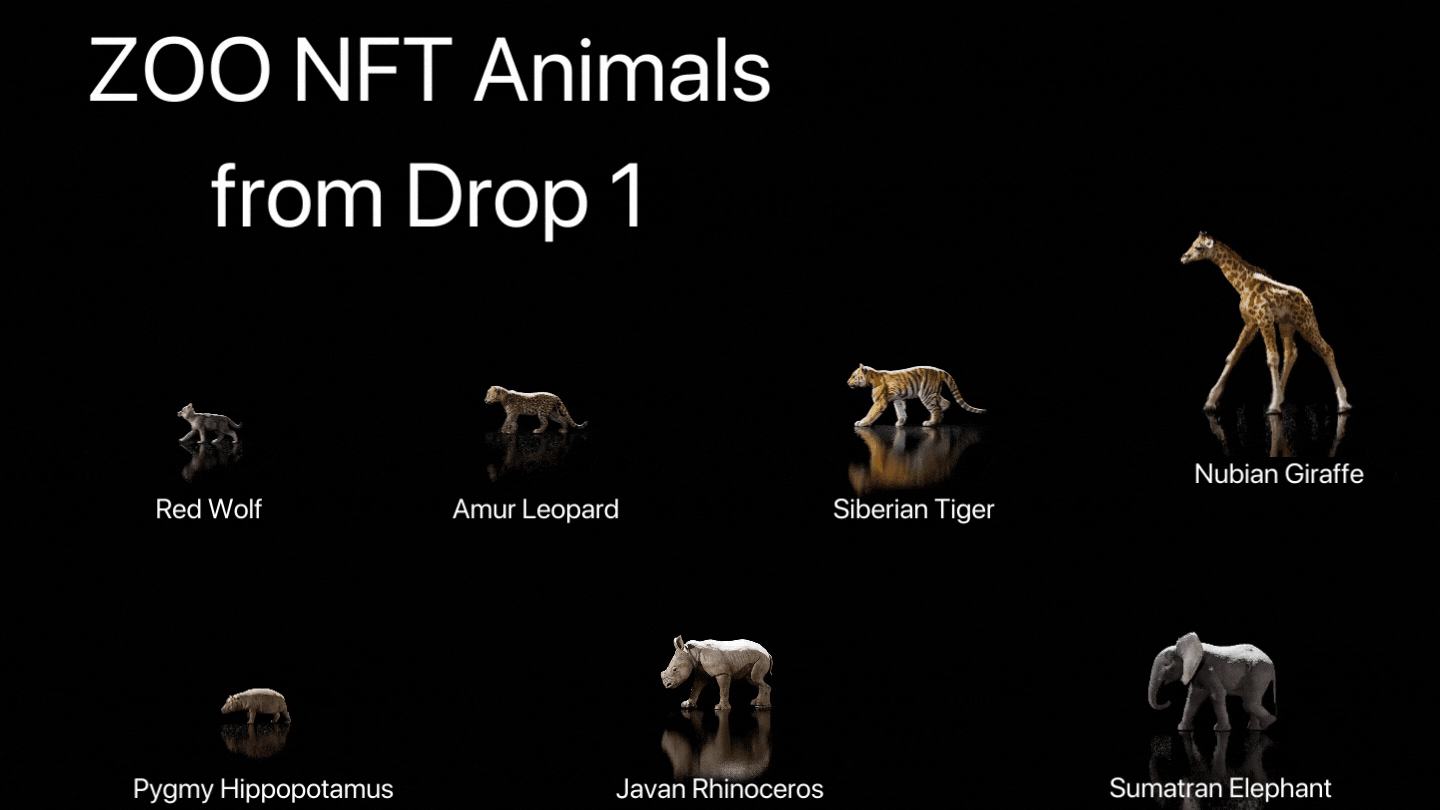
\includegraphics[width=0.85\linewidth]{figures/animals.png}
  \caption{The Zoo metaverse companions: 3D-rendered representations of endangered species, designed to inhabit AR/VR/metaverse environments.}
  \label{fig:metaverse-animals}
\end{figure}

NFT animals can be interacted with in 3 dimensions on any mobile or desktop device, by any user --- whether they own an NFT or not --- on our website. Augmented Reality (AR) capabilities allow any NFT holder to bring our NFT animals to life in their physical environments. Further functionality for NFT owners will be available after the release of our iOS/Android AR companion app, and as future upgrades and features get added.

Virtual Reality (VR) capabilities allow users who own our NFT animals to view and interact with them while immersed in VR --- in our own first-party software offerings, but also in licensing and partnership opportunities with other VR/metaverse platforms. Animals are designed to be adapted and integrated into the broader metaverse, including partnerships in development and endless possibilities as the move to the metaverse accelerates.

The animals are also literal stores of value through the innovative way our NFTs can be \emph{fed}, increasing their stored value by collateralizing them with not just \$ZOO tokens but many other popular cryptocurrencies. They grow, hatching from an NFT egg as a baby, eventually changing physical form, stats, APY, and value according to what they are fed. New functionality is added as advances in AI and emotional intelligence make it possible.

\subsection{Comparison: Why Zoo}

Zoo is a cute new game that ties witty finance strategies into a metaphor that is a Tamagotchi-like game. Tamagotchi was a handheld digital pet first released in Japan in 1996 by Bandai. The virtual pet could be cared for by inputting commands on a keychain-sized device, which would simulate the actions in Tamagotchi's digital world. The original release was extremely popular, with over 80 million units sold worldwide.

The vast majority of NFT-gaming projects lack seven key elements that Zoo provides:

\begin{itemize}
  \item A clear path to ROI through our unique approach to staking and making NFTs into stores of value, unlike those currently on the market.
  \item Universal demographic appeal: animals are subject matter that resonates across age groups.
  \item Open-source ethos: products and platforms can be built upon by an endless number of partners and sponsors.
  \item Liquidity protection through pooling mechanisms, high staking rewards, credit-card on-ramps to leverage Zoo assets, and a continuous stream of upgrades.
  \item Tax design that pumps liquidity back into the pool. For every transaction there is a tax: 4\% to the DAO, 4\% back to liquidity.
  \item DAO governance with holographic consensus, quadratic voting, aged staking, and weighted PoS.
  \item Artificially intelligent NFTs: Zoo Labs NFTs use AI and emotional intelligence to be a sort of digital pet for a multi-generational audience to play with from their mobile devices.
\end{itemize}

\section{Roadmap}
\label{sec:roadmap}

\textit{The future is filled with immersive upgrades, emotionally intelligent NFT animals, expanded metaverse lands, play-to-earn games, partnerships with celebrities, and a captivating VR/AR app and more.}

At Zoo Labs, we are set on a journey towards creating a more vibrant, immersive, and interactive NFT universe. The roadmap for our future upgrades includes features that will redefine the user experience and extend the scope of engagement with NFT animals.

We envision NFT animals not as static digital assets, but as dynamic, emotionally intelligent beings that users can interact with in the metaverse. Our planned integration of AI lets these animals understand and reciprocate emotions, evolving into emotionally intelligent avatars and creating a tapestry of emotional connection that transcends the digital divide.

We are also working towards enhancing the gaming experience by introducing mini-games and expanding our metaverse lands. The introduction of special powers and play-to-earn games offers exciting new ways for users to engage and earn rewards. Through our partnership with the Lux blockchain, players will have the opportunity to collect and redeem gold and silver coins, adding another layer of engagement and incentive.

Future upgrades also encompass new animals, including extinct species and mythical creatures, broadening the scope of our NFT animal universe. Imagine the thrill of owning and interacting with creatures that have long been extinct or only exist in mythology. Collaborations with celebrities and influencers for animal collections will create a unique cross-over between the world of entertainment and digital collectibles.

Visual differentiation includes unique animal traits such as horns, double heads, and wings, alongside a variety of skins and powers. Each NFT animal is as unique as its owner. Finally, we will launch an interactive VR/AR pet app that responds emotionally and serves as a personalized AI-powered emotional support companion.

The DAO will oversee all game functions, manage the treasury, forge partnerships, and allocate rewards for each animal. Decentralized governance ensures fair and transparent operations, strengthening the community's trust and engagement.

\subsection{Future Game Interface}

The Zoo Labs gaming landscape is composed of floating islands in the vast cosmos, each distinct and teeming with life. Each island mirrors the unique attributes of the NFT animals inhabiting them, creating diverse ecosystems waiting to be explored.

In this realm, users embody their NFT animals, experiencing the world through the animal's eyes. Engage in play-to-earn games, navigate captivating environments, and participate in quests and treasure hunts. Beyond entertainment, these adventures offer a way to earn valuable rewards.

The Zoo Labs universe is also a thriving social space where users can connect with friends and players from around the globe. Together they explore vibrant habitats, participate in games, and share the joy of discovery. Adding to the charm are the intelligent avatar animals, AI-powered companions that bring social engagement: avatars capable of learning, adapting, and reacting that make the digital experience feel more personal.

\subsection{Play-and-Earn Games}

\subsubsection{Coin Runner}

\textit{The ultimate quest for valuable gold and silver coins.}

Embark on a thrilling adventure through the Zoo Labs temple, where every coin collected brings users one step closer to real-world gold and silver rewards. Choose one of your Zoo animals to play with --- each with unique abilities and skills. Start your run through the captivating Zoo Labs temple, avoiding obstacles and outwitting cunning adversaries. Collect small gold and silver nuggets, representing the smallest denomination of gold/silver, as you dash through the temple's winding paths. Look out for larger coins, which hold greater value and signify the second-largest denomination. Seek out the ultimate prize: the coveted bullion bar, representing the most valuable form of gold and silver in the game. Use your collected coins strategically to unlock power-ups, upgrades, and new animals. Compete on the global leaderboards. All rewards are redeemable for physical assets or transferable on the Zoo Market or a secondary marketplace.

\subsubsection{Memory Bridge}

An exhilarating game set in the immersive Zoo Labs Metaverse. Join your Zoo animals on an adventure across a treacherous bridge, where quick thinking and sharp memory skills are the keys to success. Select one of your Zoo animals as game companion. Memorize the pattern of bricks connecting the bridge from left to right. As the game progresses, the bridge becomes longer, increasing the challenge and the potential rewards. The player has only 4 seconds per level to step on the correct brick and prevent the bridge from crumbling into the lava below. Choosing the wrong brick results in the animal falling and the game restarting. Successfully completing each level earns valuable rewards including rare items, tokens, and special powers for the Zoo animal --- all redeemable for real-world assets, ranging from exclusive merchandise to unique experiences.

\section{Partnerships}
\label{sec:partnerships}

\textit{Future partnerships, upgrades, and game features: building a thriving community.}

At Zoo Labs, we believe in the power of collaboration and community-driven initiatives. As we pave the way for a brighter future of conservation and environmental stewardship, the following plans for future partnerships, upgrades, and game features will fuel the growth of our community.

\paragraph{Collaborating with non-profits.} Our commitment to protecting endangered species and preserving their habitats extends beyond the boundaries of Zoo Labs. We are actively seeking partnerships with non-profit organizations that share our mission and values. By combining resources, expertise, and networks, we amplify our efforts in fundraising campaigns, educational programs, and joint conservation projects.

\paragraph{Empowering the DAO.} The decentralized autonomous organization (DAO) lies at the core of Zoo Labs, empowering community members to actively participate in shaping the future. Through the DAO, community members vote on partnerships, game upgrades, and the direction of Zoo Labs. Decentralized governance fosters inclusivity, transparency, and collective ownership.

\paragraph{Continuous game enhancements.} Our team is continuously enhancing the Zoo Labs game experience: new animal species, expanded habitats, and interactive gameplay elements that immerse you in adventure and discovery.

\paragraph{Cross-platform integration.} We are actively exploring cross-platform integration, collaborating with other blockchain-based gaming platforms, virtual-reality experiences, and even real-world events. By forging these connections, we extend our community and provide players with a truly interconnected experience.

\paragraph{The power of decentralization.} Zoo Labs embraces the decentralized nature of blockchain technology and recognizes its transformative potential. Decentralization ensures that decisions are made collectively, without the need for intermediaries or centralized control. This empowers individuals to contribute, govern, and shape the future of Zoo Labs.

\section{Open Source}
\label{sec:open-source}

By making Zoo open-source, developers can build on top of Zoo and use the \$ZOO token as their projects' virtual utility token, or build other games and NFT platforms parallel to our codebase.

This allows the utility of the \$ZOO token to go beyond our own project and become the virtual utility token of a potentially endless number of additional projects, creating enormous potential that is not possible without alignment to open-source ideology. Furthermore, our project's strong foundational support in the field of education will be an element that shines through the use of open-source resources. Educational content will be created and curated by the Zoo Foundation's resident Director of Education.

In Q2 2022, Zoo will be working with our partners in conservation to establish content shared through the Zoo Foundation in an open-source format. This educational content, aligned to nationally recognized learning standards for grade levels K--12, will be free to schools around the US. Schools will be encouraged to share the results of their time spent working with the materials we create in a repository of open-source materials on the Zoo Foundation's website.

Our developers are dedicated to improving the future of the world. We cannot wait to see what future developments come out of our community. The possibilities are endless, and they begin with community engagement. Join us on GitHub.

\section{Open AI Protocol --- The Founding Vision}
\label{sec:open-ai-protocol}

The intelligent avatars described in this paper are not a feature bolted onto NFT collectibles --- they are the founding vision of Zoo Labs as an open AI protocol for animal preservation, education, and emotional companionship. This section makes that founding vision explicit.

Zoo Labs was conceived as an \emph{open AI protocol}: a protocol where the conversational and emotional intelligence of every digital animal is composable, swappable, and governed by the community rather than a single vendor. Three principles ground that protocol:

\begin{enumerate}
  \item \textbf{Open weights, open prompts, open data.} The personality prompts shipped with every animal (Section~\ref{sec:ai-assistant}) are public, auditable, and modifiable by their owners. The training corpus for any future custom model is contributed by the community of holders. There is no proprietary black box at the heart of the experience.
  \item \textbf{Conservation as the alignment objective.} The \emph{telos} of the AI protocol is the preservation of endangered species. Every conversation with an animal avatar is an opportunity to deepen empathy and direct economic value back into the on-chain conservation treasury managed by the Zoo DAO.
  \item \textbf{Multi-modal embodiment.} The same animal AI agent is reachable across surfaces --- 2D web, AR, VR, and metaverse --- through a consistent personality and memory layer. The protocol's reach grows with the metaverse rather than being trapped on any one platform.
\end{enumerate}

These principles deliberately mirror the AI/blockchain/metaverse intersection that the rest of the paper details. The Open AI Protocol is the unifying thesis: an animal NFT is simultaneously a financial primitive (a collateralized liquidity position), a conservation token (proceeds flow to non-profit partners via the DAO), and an AI agent (an emotionally intelligent companion). All three modalities are open and composable. We believe this combination is what makes Zoo durable beyond any single market cycle of either crypto or AI.

\section{2025 Update --- Securities, Quantum-Secure Settlement, Holographic DAO, and Open Information}
\label{sec:2025-update}

\textit{This section is an editorial addendum dated 2025-12-15, four
years after the original whitepaper. It exists to surface five planks
that descend from the founding vision but were not specified in the
2021 text. The original document above is unchanged; this addendum is
the canonical bridge from the founder vision to the activation state
on 2025-12-25.}

\subsection{Updated team and mission (2025)}

\textbf{Founder}: Antje Worring (author of this October~31, 2021
whitepaper). \textbf{Chief Scientist}: Zach Kelling. \textbf{Mission} (as
of 2025-12-15): \emph{An open AI protocol for research aligned with
environment-saving, endangered AI, and the intersection of AI,
blockchain, metaverse, and gaming.} Full team page is the canonical
\texttt{team.md} in the Zoo \textsc{zip} repository. Allied
organizations: Lux Network (chain infrastructure), Hanzo AI (Techstars
'17, AI compute and Zen LM co-development), and a regulated securities
partner (exclusive partner for retail-scale digital-securities trading).

\subsection{\$113 trillion digital-securities market}

The total addressable market for digital securities globally is
estimated at approximately \textbf{\$113 trillion} (BIS / WFE 2025
estimates of global capitalization across equities, fixed income,
derivatives, and tokenized real-world assets). Zoo positions itself as
the open AI / wildlife / metaverse layer in this stack. Lux provides
the regulated chain infrastructure. \textbf{A regulated securities partner} is Zoo's
exclusive partner for retail-scale securities trading, carrying the
regulated ATS / broker-dealer / transfer-agent perimeter.

\paragraph{Tagline.} \emph{Robinhood-style capabilities for everyone ---
actually make money like the 1\% finally.}

\paragraph{Concrete capabilities.} Zero-commission trading, fractional
shares to the cent, instant settlement on Quasar 3.0, tokenized
real-world securities (stocks, bonds, commodities, REITs, private
equity), 24/7 markets, and a public verifiable order book. Compliance
(KYC, AML, suitability, best execution) lives at the regulated securities partner's
perimeter; the chain is the audit-eligible settlement layer.

\paragraph{Honest framing.} \$113T is a market-size figure, not a
Zoo-specific TVL. Zoo Labs Foundation is a 501(c)(3) and does not
operate a regulated market center; the regulated securities partner does.

\subsection{Quantum-secure settlement (Quasar 3.0)}

Every securities trade, every Zoo block, every NFT mint, and every DAO
vote settles under \textbf{Quasar 3.0} (Lux LP-020). Quasar 3.0
composes three independent cryptographic hardness assumptions:

\begin{itemize}[nosep,leftmargin=1.2em]
\item BLS12-381 aggregate signature (classical), Lux LP-075.
\item Corona Ring-LWE threshold signature (post-quantum lattice),
   Lux LP-073.
\item ML-DSA-65 identity proof via Z-Chain Groth16 rollup
   (post-quantum lattice with succinct proof), Lux LP-070.
\end{itemize}

An adversary must break \emph{all three} to forge a Lux/Zoo block. A
BLS compromise on Q-day does not break finality: the Corona +
ML-DSA pair stays secure. M-Chain (Lux LP-019) holds threshold custody
of governance and settlement keys; F-Chain (Lux LP-013) provides FHE
substrate. The retail user can therefore truthfully say: trade
post-quantum-safe, custody post-quantum-safe, audit-trail
post-quantum-safe.

\subsection{Homomorphic / Holographic Consensus DAO}

The Zoo DAO described in §19 of the 2021 text now formalizes as a
\emph{homomorphic} (votes tallied while encrypted via F-Chain FHE,
Lux LP-013) and \emph{holographic} (every sub-DAO is structurally a
copy of the meta-DAO; per-LLM chains, research verticals, and regional
chapters all inherit the same governance topology) consensus DAO.

Voting weight is

\[
\text{weight}(p) \;=\; \alpha \cdot a_p \;+\; \beta \cdot i_p \;+\; \gamma \cdot c_p \;+\; \delta \cdot s_p
\]

\noindent with $\alpha + \beta + \gamma + \delta = 1$, where the four
axes are advocacy ($a_p$), involvement ($i_p$), contribution ($c_p$),
and token stake ($s_p$). Default initial weights at 2025-12-25:
$(0.20, 0.30, 0.40, 0.10)$. Token stake is bounded at 10\% to prevent
plutocracy. Anti-Sybil: contribution and involvement scores require
TEE attestation through A-Chain (Lux LP-134); advocacy must be on
attestation-rooted social platforms. Threshold custody of governance
keys lives on M-Chain MPC (Lux LP-019).

\subsection{Democratized end-to-end access to information}

The Open AI Protocol named in §\ref{sec:open-ai-protocol} now operates
as an end-to-end-verifiable pipeline:

\begin{enumerate}[nosep,leftmargin=1.4em]
\item User --- proves eligibility via zero-knowledge selective
   disclosure (Z-Chain Groth16 attestations).
\item Model --- weights, architecture, and training-data lineage all
   committed on-chain via Zoo per-LLM chains.
\item Data --- every training shard's hash is on the receipts tree;
   contributors are attributable.
\item Output --- every inference call produces a TEE-attested receipt
   anchored on A-Chain via the Hanzo AI Chain.
\item Reward --- royalties flow back along the contribution graph
   automatically.
\end{enumerate}

Closed labs (OpenAI, Anthropic) treat weights, data, and architecture
as competitive secrets. Zoo treats them as public goods whose
provenance is the protocol. This is the durable distinction between
the open AI protocol named in the 2021 founding vision and the
proprietary AI services that came after.

\subsection{Cross-references}

\begin{itemize}[nosep,leftmargin=1.2em]
\item Companion paper: \emph{Zoo 2025: Digital Securities,
   Quantum-Secure Settlement, and the Holographic Consensus DAO}
   (full-length treatment of the five planks).
\item Companion paper: \emph{Zoo Per-LLM Chains: One Sovereign Chain
   per Model}.
\item Lux LP-020 (Quasar 3.0), LP-013 (F-Chain), LP-019 (M-Chain),
   LP-070 (ML-DSA), LP-073 (Corona), LP-075 (BLS), LP-105 (Quasar
   3.0 paper), LP-134 (A/B/M/F topology).
\item Hanzo AI Chain whitepaper.
\item Zoo \textsc{zip-0017} (DAO governance), \textsc{zip-0026}
   (reputation), \textsc{zip-0570} (impact thesis).
\end{itemize}

\medskip
\noindent\textit{Editorial addendum closes 2025-12-15.}


\clearpage
\section*{Colophon}
\addcontentsline{toc}{section}{Colophon}

This document is a faithful reconstruction of the Zoo Labs Foundation whitepaper, originally published online at \url{https://zoolabs.gitbook.io/whitepaper/}. The reconstruction was performed on 2025-12-15 to preserve the founder vision in archival LaTeX form. Every section corresponds to a page in the source whitepaper. All images were retrieved from the live gitbook CDN and are reproduced here under the Zoo Labs Foundation's own publication.

The original publication date of October 31, 2021 reflects when Antje Worring first articulated this vision as the canonical founder document for the Zoo Labs Foundation.

For the most current version of the Zoo ecosystem, including post-2021 evolutions of the AI protocol and DAO governance, see the companion papers in the Zoo Labs research series at \url{https://zoo.ngo/papers}.

\end{document}
